


% \graphicspath{{Chap2/plots/}}
The transition matrix, or T-matrix, relates the multipole coefficients of the scattered field of an object to the multipole coefficients of the field incident on the object. The method was pioneered by Waterman \cite{waterman1965matrix}.  A T-matrix can represent the scattering solution of a single object or a collection of objects, \cite{chew1995waves}. Deriving or computing the elements of a T-matrix is its own subject, but simple objects admit analytic solutions. This chapter gives the basic definition of the T-matrix and instructions for rotation. Then equations and routines for the T-matrix elements of dielectric and metal spheres are provided. Derivations and routines are then provided to convert between a T-matrix and an S-matrix. Finally, we give expressions for different radar cross sections in terms of the T-matrix and evaluate these for spheres.


\section{Definition}

The incident field is expanded in regular spherical wave functions around the object, and the scattered field is expanded in radiating wave functions. The harmonic sums are written in matrix notation as
\begin{eqnarray}
\bb{E}_{inc}(\br) &=& \onebytwo{\textit{Rg}\bb{M}^t(k,\br)}{\textit{Rg}\bb{N}^t(k,\br)}\twobyone{\bb{a}}{\bb{b}} \\
\bb{E}_{sca}(\br) &=& \onebytwo{\bb{M}^t(k,\br)}{\bb{N}^t(k,\br)}\twobyone{\bb{c}}{\bb{d} \label{tmatrixesca} } 
\end{eqnarray}

The expression for the incident field is valid everywhere, while the scattered field is only valid outside the smallest radius that encloses the object or collection of objects. In other words, a T-matrix does not model the scattering solution within an object region.  Next, define the sub-matrices that relate the expansion coefficients between the $\bb{M}$ and $\bb{N}$ harmonics as  
\begin{equation}
\twobyone{\bb{c}}{\bb{d}} = \twobytwo{\overline{\bb{T}}^{MM}}{\overline{\bb{T}}^{MN} }{\overline{\bb{T}}^{NM}}{\overline{\bb{T}}^{NN}} \twobyone{\bb{a}}{\bb{b} \label{Tmatrixdef} }
\end{equation}


An object and its T-matrix can be rotated using the rotation matrix for spherical harmonics. Given an object T-matrix, the T-matrix of the object rotated by ZXZ Euler angles $(\alpha,\beta,\gamma)$ is
\eq{\twobytwo{\overline{\bb{T}}^{'MM}}{\overline{\bb{T}}^{'MN} }{\overline{\bb{T}}^{'NM}}{\overline{\bb{T}}^{'NN}} = 
\twobytwo{\bb{D}^*}{0}{0}{\bb{D}^*}
\twobytwo{\overline{\bb{T}}^{MM}}{\overline{\bb{T}}^{MN} }{\overline{\bb{T}}^{NM}}{\overline{\bb{T}}^{NN}} 
\twobytwo{\bb{D}}{0}{0}{\bb{D}} }

\noindent where $\bb{D}$ describes the inverse rotation and $\overline{\bb{T}}'$ is the T-matrix of the rotated object as seen from the fixed frame. The field first viewed from the frame of the rotated object, then the T-matrix is applied in its natural frame, last the perspective is rotated back to the fixed frame (an inverse rotation in the opposite direction, i.e., a forward rotation, $\bb{D}^*$.)



%The rule of thumb for the number of unique $(l,m)$ harmonics needed to represent the scattered field of an object with the multipole expansion is $O(kd)$, where $k$ is the background wavenumber, and $d$ is the largest dimension of the object. Alternately, $d$ can be thought of as the diameter of the smallest sphere enclosing the object.  The total number harmonics up to $L$ all $m$ is 
%
%\eq{N = \sum_{l=1}^{L} \sum_{m=-l}^l 1 = L^2 + 2L}
%
%Then solving the quadratic for $L$ we get, roughly, 
%
%\eq{L \approx 2 \sqrt{kd  + 1} - 1}

%which is rounded up.  

\clearpage
\newpage
\section{Object T-matrix}

This section derives the T-matrix for several simple objects.

\subsection{Dielectric Sphere}
\label{sec:tmatrixsphere}
Let a sphere of radius $a$ be centered at the origin with outer and inner regions having wavenumbers $k_1$ and $k_2$, respectively.  The incident, scattered, and total electric fields are expanded in terms of vector spherical wave functions. The regular form of the wave functions is used for the incident everywhere and the total field inside the sphere, while the singular form is used for the scattered field outside of the sphere. 
\begin{eqnarray}
\bb{E}_{inc}(\br) &=& \onebytwo{\textit{Rg}\bb{M}^t(k_1,\br)}{\textit{Rg}\bb{N}^t(k_1,\br)}\twobyone{\bb{a}}{\bb{b}}, \quad \forall \ \br \\
\bb{E}_{sca}(\br) &=& \onebytwo{\bb{M}^t(k_1,\br)}{\bb{N}^t(k_1,\br)}\twobyone{\bb{c}}{\bb{d}}, \quad \br \ge a \\
\bb{E}_{tot}(\br) &=& \onebytwo{\textit{Rg}\bb{M}^t(k_2,\br)}{\textit{Rg}\bb{N}^t(k_2,\br)}\twobyone{\bb{e}}{\bb{f}}, \quad \br \le a
\end{eqnarray}

\vspace{-2mm}
The magnetic fields are found by taking the curl of each expression (i.e., Faraday's law) and applying the curl relations for vector spherical wave functions. For example, the scattered magnetic field is 
\begin{equation}
\bb{H}_{sca}(\br) = \frac{k}{i\omega\mu}\onebytwo{\bb{N}^t(k,\br)}{\bb{M}^t(k,\br)}\twobyone{\bb{c}}{\bb{d}}
\end{equation}

Boundary conditions require that the tangential electric and magnetic fields at $r=a$ must be equal
\begin{eqnarray}
\hat{\br}\times\bb{E}_{tot} &=& \hat{\br}\times\bb{E}_{inc} + \hat{\br}\times\bb{E}_{sca} \label{rcrossescat} \\
\hat{\br}\times\bb{H}_{tot} &=& \hat{\br}\times\bb{H}_{inc} + \hat{\br}\times\bb{H}_{sca} \label{rcrosshscat}
\end{eqnarray}

We want to express the total and scattered field coefficients in terms of the incident field coefficients. We outline the steps and state the result. Left dot \eqref{rcrossescat} and \eqref{rcrosshscat} by $\hat{\bb{M}}(k_1,\br)$ and by $\hat{\bb{N}}(k_1,\br)$, respectively, where the caret, $\hat{}$, means the angular harmonics are conjugated.  Apply the vector identity that exchanges dot and cross product, evaluate at $r=a$, and integrate over the unit sphere. Orthogonality will pick out the $l$ harmonics. Solve the resulting system of equations, and after some simplifications, including use of the Wronskian, we get the following relations between the coefficients.
\begin{equation}
c_{lm} = -a_{lm}\dfrac{\mu_2 j_l(k_2a)\left[k_1aj_l(k_1a)\right]' - \mu_1 j_l(k_1a) \left[k_2aj_l(k_2a)\right]'}{\mu_2 j_l(k_2a) [k_1ah_l^{(1)}(k_1a)]' - \mu_1 h_l^{(1)}(k_1a)\left[k_2aj_l(k_2a)\right]'} \label{clmalm}
\end{equation}

\begin{equation}
d_{lm} = -b_{lm}\dfrac{\epsilon_2 j_l(k_2a)\left[k_1aj_l(k_1a)\right]' - \epsilon_1 j_l(k_1a) \left[k_2aj_l(k_2a)\right]'}{\epsilon_2 j_l(k_2a) [k_1ah_l^{(1)}(k_1a)]' - \epsilon_1 h_l^{(1)}(k_1a)\left[k_2aj_l(k_2a)\right]'} \label{dlmblm}
\end{equation}

\begin{equation}
e_{lm} = a_{lm}\dfrac{i\mu_1}{k_1a}\dfrac{1}{ \mu_2 j_l(k_2a) [k_1ah_l^{(1)}(k_1a)]' - \mu_1 h_l^{(1)}(k_1a)\left[k_2aj_l(k_2a)\right]' } \label{elmalm}
\end{equation}

\begin{equation}
f_{lm} = b_{lm}\dfrac{i\epsilon_2}{k_2a}\dfrac{1}{\epsilon_2 j_l(k_2a) [k_1ah_l^{(1)}(k_1a)]' - \epsilon_1 h_l^{(1)}(k_1a)\left[k_2aj_l(k_2a)\right]' } \label{flmblm}
\end{equation}

\noindent where $a$ is the radius, $k_1$ is the wavenumber outside the sphere, $k_2$ is the wavenumber inside the sphere, either given by 
\eq{k = \omega\sqrt{\mu\epsilon} = \dfrac{\omega}{c} \sqrt{\mu_r \epsilon_{rc}}}
\eq{\epsilon_{rc} = \epsilon_r + i\dfrac{\sigma}{\omega\epsilon_o}}

\noindent where $\omega$ is the natural frequency, $c$ is the speed of light in vacuum, $\mu$ is the magnetic permeability, $\mu_r$ is the relative permeability, $\epsilon$ is the dielectric permittivity, $\epsilon_{rc}$ is the relative complex permittivity, $\epsilon_r$ is the real part of the relative permittivity, $\sigma$ is the conductivity, and $\epsilon_{o}$ is the permittivity of free space.  The Bessel derivatives apply to the argument $x = ka$ as
\begin{equation}
[ x z_l(x)]' = z_l(x) + x z_l'(x) 
\end{equation}

Equations \eqref{clmalm} and \eqref{dlmblm} give the scattered field coefficients, while \eqref{elmalm} and \eqref{flmblm} give the coefficients for the total field inside the sphere. Dividing \eqref{clmalm} and \eqref{dlmblm} by $a_{lm}$ and $b_{lm}$, respectively, gives the T-matrix elements for the dielectric sphere. 
\begin{eqnarray}
T^{MM}_{lmlm}  &=& \dfrac{c_{lm}}{a_{lm}} \label{tmmsphere} \\
T^{NN}_{lmlm} &=&  \dfrac{d_{lm}}{b_{lm}}  \label{tnnsphere}\\
T_{lmlm}^{MN} &=& 0 \\
T_{lmlm}^{NM} &=& 0 
\end{eqnarray}

This T-matrix is diagonal, so there is no mode-mixing, and the elements are only a function the degree $l$, which are copied for all $m$ at that degree. 

The routine \texttt{tmatrixDielectricSphere} gives the T-matrix elements of a dielectric sphere up to maximum degree $L$ all $m$. It takes as input the maximum degree harmonic $L$, sphere radius, and wavenumbers and inside and outside the sphere. The permeabilities are optional, but if nonzero, must also be included in the wavenumbers.  

{\footnotesize
\VerbatimInput{\code/Tmatrix/tmatrixDielectricSphere.m}
}



\subsection{PEC Sphere}

The T-matrix for a perfect electrical conductor (PEC) sphere is found by taking $\epsilon_2 \rightarrow \infty$ and/or $\mu_2 \rightarrow 0$ in \eqref{tmmsphere} and \eqref{tnnsphere}.  The result is
\begin{eqnarray}
T_{lmlm}^{MM} &=& -\dfrac{j_l(ka)}{h_l^{(1)}(ka)} \\
T_{lmlm}^{NN} &=& -\dfrac{[k a j_l(ka)]'}{[k a h_l^{(1)}(ka)]'} \\
T_{lmlm}^{MN} &=& 0 \\
T_{lmlm}^{NM} &=& 0 
\end{eqnarray}

\noindent where $k$ is the background wavenumber.  The negative sign is the 180 degree phase flip familiar from 1D scattering from a PEC boundary. 

The routine \texttt{tmatrixPECSphere} gives the T-matrix elements of a PEC sphere up to maximum degree $L$ all $\pm m$.  

{\footnotesize
\VerbatimInput{\code/Tmatrix/tmatrixPECSphere.m}
}

%\subsection{Multilayered Dielectric Sphere}
%\subsection{PEC Cylinder}
%\subsection{Dielectric Cylinder}
%\section{Multilayered Dielectric Sphere with PEC Core}

\clearpage
\newpage
\section{Extended Boundary Condition Method}

The extended boundary condition method (EBCM) is a technique to compute the T-matrix of a bounded, homogenous object that has an arbitrary or irregular surface. For example, this has been used to determine the T-matrix of short cylinders in \cite{duan2015experimental}.  While analytically generic, the EBCM is usually not accurate for highly elongated objects or objects with large concavities. We outline the derivation, comment on the computation, and provide a routine to compute the solution.

\paragraph{Formulation}
The EBCM makes use of the extinction theorem to express fields both inside and outside the object in terms of an integral over the surface of the object, \cite{chew1995waves}. The geometry is shown in Figure \ref{geoebcm}. The extended boundaries are two virtual surfaces, $S_1$ and $S_2$, that are contained in the volumes, $V_1$ and $V_2$, respectively, but do not intersect the actual surface, $S$. $S_1$ and $S_2$ are used to decide the form of the addition theorem for the dyadic Green's function. The fields tangent to $S$ are expanded in terms of vector spherical wave functions, after which the incoming and outgoing field coefficients can be related and the T-matrix found.  


\begin{figure}[H] 
   \centering
   \includegraphics[width=2.2in]{Tmatrix/Figures/ebcm} 
   \caption{Geometry for the Extended Boundary Condition Method.}
   \label{geoebcm}
\end{figure}

The surface integral equations used for the EBCM are \cite{chew1995waves,duan2015experimental}, 
\begin{align}
\bb{E}_{inc}(\br) &= -\int_S dS'\left( i \omega \mu_1 \G{1} \cdot \hat{n}' \times \bb{H}_1(\br') + \left[\nabla\times \G{1} \right] \cdot \hat{n}' \times \bb{E}_1(\br') \right), \quad \br \in V_2  \label{ebcmSIEV2}\\
0 &= -\int_S dS'\left( i \omega \mu_2 \G{2} \cdot \hat{n}' \times \bb{H}_2(\br') + \left[\nabla\times \G{2} \right] \cdot \hat{n}' \times \bb{E}_2(\br') \right), \quad \br \in V_1  \label{ebcmSIEV1}
\end{align}

\noindent where $\hat{n}'$ is the outward pointing surface normal (the leading minus sign is missing in \cite{chew1995waves}, and \eqref{dyadicGreenscurlprime} has been applied to the curl). The dyadic Green's functions are evaluated at the wavenumbers $k_1$ and $k_2$ of the outer and inner regions, respectively.  Note, each equation is only valid when the observation point, $\br$, is in the region of the opposite wavenumber. 

The addition theorem for the dyadic Green's function, \eqref{dyadicgreensaddition}, is used to expand $\G{1}$ and $\G{2}$ on the virtual surfaces, $S_2$ and $S_1$, respectively, according the rule that the regular form of the wave functions are used for the smaller of $\br$ or $\br'$.  Therefore,
\ea{\G{1} &=& ik_1\sum_{l=1}^{\infty}\sum_{m=-l}^l \textit{Rg}\M{k_1,\br}\Mhat{k_1,\br'} + \textit{Rg}\N{k_1,\br}\Nhat{k_1,\br'}, \quad \br \in S_2  \label{ebcmg1} \\
\G{2} &=& ik_2\sum_{l=1}^{\infty}\sum_{m=-l}^l \M{k_2,\br}\textit{Rg}\Mhat{k_2,\br'} +\N{k_2,\br} \textit{Rg}\Nhat{k_2,\br'}, \quad \br \in S_1 \label{ebcmg2} }

%To accommodate the outer product, we apply the following curl relation 
 %\eq{\nabla' \times \G{ } = -\nabla \times \G{ } }
 
\noindent where $\hat{\ }$ means conjugate of the angular function. The dyad is formed by the outer product of the components of the wave functions, where the left vector is unprimed and the right vector is primed. The vector spherical wave functions are fully normalized. The curl in \eqref{ebcmSIEV2} and \eqref{ebcmSIEV1} must be applied to the first vector of the outer product in \eqref{ebcmg1} and \eqref{ebcmg2}, \cite{tai1997general}, which is the reason for using the unprimed curl. The tangential fields of region 2, $\hat{n}'\times\bb{E}_2(\br')$ and $\hat{n}'\times\bb{H}_2(\br')$, are expanded as (in matrix notation) 
\vspace{-2mm}
\ea{\hat{n}'\times \bb{E}_2(\br') &=& \onebytwo{\hat{n}'\times\textit{Rg}\bb{M}^t(k_2,\br')}{\hat{n}'\times\textit{Rg}\bb{N}^t(k_2,\br')}\twobyone{\boldsymbol{\alpha}^M}{\boldsymbol{\alpha}^N} \label{ebcmE2} \\
i\omega \mu_2 \hat{n}'\times \bb{H}_2(\br') &=& \onebytwo{\hat{n}'\times \nabla' \times \textit{Rg}\bb{M}^t(k_2,\br')}{\hat{n}'\times\nabla' \times \textit{Rg}\bb{N}^t(k_2,\br')}\twobyone{\boldsymbol{\beta}^M}{\boldsymbol{\beta}^N}\label{ebcmH2} 
}

\underline{Step 1}: The first step of EBCM is to derive the relationship between the expansion coefficients $\boldsymbol{\alpha}$ and $\boldsymbol{\beta}$ subject to the constraint of \eqref{ebcmSIEV1}. This starts by substituting \eqref{ebcmg2} into \eqref{ebcmSIEV1}. The curl relations for the vector wave functions, \eqref{vswfcurlM} and \eqref{vswfcurlN}, are applied to the primed wave functions to convert the curl of the wave function into the opposite wave function times the wavenumber. The result is rearranged and expressed as an expansion of unprimed wave functions so that \eqref{ebcmSIEV1} becomes
\ea{0 &=&  \sum_{l=1}^{\infty}\sum_{m=-l}^l e_{lm} \M{k_2,\br} +f_{lm} \N{k_2,\br}  \label{ebcmg2expand}  \\
e_{lm} &=& -ik_2\int_{S_1} dS' \left[ i \omega \mu_2\textit{Rg}\Mhat{k_2,\br'}\cdot \hat{n}' \times \bb{H}_2(\br')   + k_2 \textit{Rg}\Nhat{k_2,\br'} \cdot \hat{n}' \times \bb{E}_2(\br')   \right]  \label{ebcmclm} \\
f_{lm} &=&  -ik_2\int_{S_1} dS'\left[ i \omega \mu_2 \textit{Rg}\Nhat{k_2,\br'}  \cdot \hat{n}' \times \bb{H}_2(\br')  + k_2\textit{Rg}\Mhat{k_2,\br'} \cdot \hat{n}' \times \bb{E}_2(\br') \right] \label{ebcmdlm}  }

%\ea{0 &=&  -ik_2\sum_{l=1}^{\infty}\sum_{m=-l}^l \int_S dS'\left( i \omega \mu_2 \left[ \M{k_2,\br}\textit{Rg}\Mhat{k_2,\br'} +\N{k_2,\br} \textit{Rg}\Nhat{k_2,\br'} \right] \cdot \hat{n}' \times \bb{H}_2(\br') - \right.\nonumber \\
%\ & \ &\left. \left[\nabla'\times \left[  \M{k_2,\br}\textit{Rg}\Mhat{k_2,\br'} +\N{k_2,\br} \textit{Rg}\Nhat{k_2,\br'}\right] \right] \cdot \hat{n}' \times \bb{E}_2(\br') \right)  }
%\ea{0 &=&  -ik_2\sum_{l=1}^{\infty}\sum_{m=-l}^l \int_S dS'\left( \M{k_2,\br}\left[ i \omega \mu_2\textit{Rg}\Mhat{k_2,\br'}\cdot \hat{n}' \times \bb{H}_2(\br')   +\nabla'\times\textit{Rg}\Mhat{k_2,\br'} \cdot \hat{n}' \times \bb{E}_2(\br')   \right] \right.\nonumber\\
%\ &\ & \left. +\N{k_2,\br} \left[ i \omega \mu_2 \textit{Rg}\Nhat{k_2,\br'}  \cdot \hat{n}' \times \bb{H}_2(\br')  + \nabla'\times\textit{Rg}\Nhat{k_2,\br'} \cdot \hat{n}' \times \bb{E}_2(\br') \right] \right)  }

Because \eqref{ebcmg2expand} is zero for all points $\br \in V_1$, including points at infinity, and because the wave functions are independent, $e_{lm}$ and $f_{lm}$ have to be equal to zero for all $(l,m)$. Applying the curl relations again to \eqref{ebcmH2}, then substituting \eqref{ebcmE2} and \eqref{ebcmH2} into both \eqref{ebcmclm} and \eqref{ebcmdlm}, and using a different summation index, we get
\vspace{-3mm}
\ea{e_{lm} &=& -ik_2^2 \sum_{p=1}^{\infty}\sum_{q=-p}^p \int_{S_1} dS' \left[ 
\textit{Rg}\Mhat{k_2,\br'}\cdot 
\left(\hat{n}'\times\textit{Rg}\bb{N}_{pq}(k_2,\br')\beta^M_{pq} + \hat{n}'\times\textit{Rg}\bb{M}_{pq}(k_2,\br')\beta^N_{pq} \right) \right. \nonumber \\
\ & \ & \left. + 
\textit{Rg}\Nhat{k_2,\br'} \cdot 
\left(\hat{n}'\times\textit{Rg}\bb{M}_{pq}(k_2,\br')\alpha^M_{pq} + \hat{n}'\times\textit{Rg}\bb{N}_{pq}(k_2,\br')\alpha^N_{pq} \right)
   \right]   \\
f_{lm} &=&  -ik_2^2 \sum_{p=1}^{\infty}\sum_{q=-p}^p\int_{S_1} dS'\left[  
\textit{Rg}\Nhat{k_2,\br'}  \cdot 
\left(\hat{n}'\times\textit{Rg}\bb{N}_{pq}(k_2,\br')\beta^M_{pq} + \hat{n}'\times\textit{Rg}\bb{M}_{pq}(k_2,\br')\beta^N_{pq}\right) \right. \nonumber \\
\ & \ & \left. + 
\textit{Rg}\Mhat{k_2,\br'} 
\left(\hat{n}'\times\textit{Rg}\bb{M}_{pq}(k_2,\br') \alpha^M_{pq}+ \hat{n}'\times\textit{Rg}\bb{N}_{pq}(k_2,\br')\alpha^N_{pq} \right)
\right]  }

Using the vector identity $\bb{a} \cdot (\bb{b} \times \bb{c}) = \bb{b} \cdot (\bb{c} \times \bb{a})$, and the fact that cross products of similar wave function are equal to zero, these simplify to  
\ea{e_{lm} &=& -ik_2^2 \sum_{p=1}^{\infty}\sum_{q=-p}^p \int_{S_1} dS' \hat{n}' \cdot \left[ 
 \textit{Rg}\bb{N}_{pq}(k_2,\br')\times \textit{Rg}\Mhat{k_2,\br'}  \beta^M_{pq}  + 
 \textit{Rg}\bb{M}_{pq}(k_2,\br')\times \textit{Rg}\Nhat{k_2,\br'}    \alpha^M_{pq}    
   \right] \nonumber  \\
 \ & \ &\label{ebcmelm2} \\
f_{lm} &=&  -ik_2^2 \sum_{p=1}^{\infty}\sum_{q=-p}^p\int_{S_1} dS'\hat{n}' \cdot\left[  
   \textit{Rg}\bb{M}_{pq}(k_2,\br')\times\textit{Rg}\Nhat{k_2,\br'}    \beta^N_{pq}   + 
  \textit{Rg}\bb{N}_{pq}(k_2,\br')\times\textit{Rg}\Mhat{k_2,\br'}\alpha^N_{pq}  
\right] \nonumber \label{ebcmflm2} \\}


%these can be rearranged as  
%\ea{c_{lm} &=& -ik_2^2 \sum_{p=1}^{\infty}\sum_{q=-p}^p \int_{S_1} dS' \hat{n}' \cdot \left[ 
% \textit{Rg}\bb{N}_{pq}(k_2,\br')\times \textit{Rg}\Mhat{k_2,\br'}  \beta^M_{pq} +  \textit{Rg}\bb{M}_{pq}(k_2,\br')\times \textit{Rg}\Mhat{k_2,\br'} \beta^N_{pq}  \right. \nonumber \\
%\ & \ & \left. - 
% \textit{Rg}\bb{M}_{pq}(k_2,\br')\times \textit{Rg}\Nhat{k_2,\br'}    \alpha^M_{pq} -  \textit{Rg}\bb{N}_{pq}(k_2,\br')\times \textit{Rg}\Nhat{k_2,\br'}   \alpha^N_{pq} 
%   \right]   \\
%d_{lm} &=&  -ik_2^2 \sum_{p=1}^{\infty}\sum_{q=-p}^p\int_{S_1} dS'\hat{n}' \cdot\left[  
% \textit{Rg}\bb{N}_{pq}(k_2,\br')\times\textit{Rg}\Nhat{k_2,\br'}    \beta^M_{pq} +  \textit{Rg}\bb{M}_{pq}(k_2,\br')\times\textit{Rg}\Nhat{k_2,\br'}    \beta^N_{pq}  \right. \nonumber \\
%\ & \ & \left. - 
%  \textit{Rg}\bb{M}_{pq}(k_2,\br')\times\textit{Rg}\Mhat{k_2,\br'} \alpha^M_{pq}- \textit{Rg}\bb{N}_{pq}(k_2,\br')\times\textit{Rg}\Mhat{k_2,\br'}\alpha^N_{pq}  
%\right]  }

\vspace{-3mm}
Next, choose $S_1$ to be a sphere so that $\hat{n}' = \hat{r}$. From the cross-product  relations for the vector spherical wave functions over a sphere \eqref{MNrorth1}-\eqref{MNrorth3}, the integrals will be non-zero only when $(l,m) = (p,q)$. The Bessel function products that remain are identical between the two indicies, so these can be factored from the difference. Finally, because $ \bb{M}_{lm}\times\hat{\bb{N}}_{lm} = -\hat{\bb{N}}_{lm}\times \bb{M}_{lm}$, and $ \bb{N}_{lm}\times\hat{\bb{M}}_{lm} = -\hat{\bb{M}}_{lm}\times \bb{N}_{lm}$, and using the fact that $e_{lm} = 0$ and $f_{lm}=0$, we have the constraint
%\vspace{-5mm}
\ea{0 &=&    \beta^M_{pq}  - \alpha^M_{pq}  \\
0 &=&   \beta^N_{pq}  -  \alpha^N_{pq}  }


%, \eqref{vswfcurlM} and \eqref{vswfcurlN}, and rearranging, we get
%\ea{0 &=&  -ik_2\sum_{l=1}^{\infty}\sum_{m=-l}^l \int_S dS'\left( i \omega \mu_2 \left[ \M{k_2,\br}\textit{Rg}\Mhat{k_2,\br'} +\N{k_2,\br} \textit{Rg}\Nhat{k_2,\br'} \right] \cdot \hat{n}' \times \bb{H}_2(\br') - \right.\nonumber \\
%\ & \ &\left. k_2 \left[\left[  \M{k_2,\br}\textit{Rg}\Nhat{k_2,\br'} +\N{k_2,\br} \textit{Rg}\Mhat{k_2,\br'}\right] \right] \cdot \hat{n}' \times \bb{E}_2(\br') \right), \quad \br \in V_1  }

%Using \eqref{ebcmg2} in \eqref{ebcmSIEV1}, then substituting \eqref{ebcmE2} and \eqref{ebcmH2}, and following the steps in \cite{chew1995waves}, it can be shown that $\boldsymbol{\alpha}^M = \boldsymbol{\beta}^M$ and $\boldsymbol{\alpha}^N = \boldsymbol{\beta}^N$. 

\noindent or $\boldsymbol{\alpha}^M = \boldsymbol{\beta}^M$ and $\boldsymbol{\alpha}^N = \boldsymbol{\beta}^N$ for all harmonics.  

%In \cite{chew1995waves,duan2015experimental}, the same coefficient relations do not have a minus sign, but this sign comes from the fact that the cross products of the pairs of wave functions in \eqref{ebcmelm2} and \eqref{ebcmflm2} are reversed. 

\underline{Step 2}: The second step of the EBCM is to use \eqref{ebcmSIEV2} to derive a relationship between expansion coefficients of the incident and tangential fields. This starts by expanding the incident field as regular waves in region 2 using the wavenumber of region 1
\eq{\bb{E}_{inc}(\br) = \onebytwo{\textit{Rg}\bb{M}^t(k_1,\br)}{\textit{Rg}\bb{N}^t(k_1,\br)}\twobyone{\bb{a}}{\bb{b}}, \quad \br \in V_2 \label{ebcmeinc2}}
 
Substituting \eqref{ebcmeinc2} and \eqref{ebcmg1} into \eqref{ebcmSIEV2}, applying the curl, and matching like harmonics of the unprimed wave functions, the incident field expansion coefficients are written in terms of the tangential fields as
\ea{a_{lm} &=& -ik_1 \int_S dS'\left( i \omega \mu_1  \Mhat{k_1,\br'}   \cdot \hat{n}' \times \bb{H}_1(\br') +   k_1\Nhat{k_1,\br'}  \cdot \hat{n}' \times \bb{E}_1(\br') \right) \label{ebcmalm1} \\
b_{lm} &=& -ik_1\int_S dS'\left( i \omega \mu_1   \Nhat{k_1,\br'}\cdot \hat{n}' \times \bb{H}_1(\br') +    k_1\Mhat{k_1,\br'}  \cdot \hat{n}' \times \bb{E}_1(\br') \right) \label{ebcmblm1}}

Because the tangential fields of region 1 and region 2 must be equal on $S$, then $\hat{n}'\times \bb{E}_1(\br')$ and $\hat{n}'\times \bb{H}_1(\br')$ can be expanded using \eqref{ebcmE2} and \eqref{ebcmH2}, respectively. The tangential fields of region 1 are then
\ea{\hat{n}'\times \bb{E}_1(\br') &=&\onebytwo{\hat{n}'\times\textit{Rg}\bb{M}^t(k_2,\br')}{\hat{n}'\times\textit{Rg}\bb{N}^t(k_2,\br')}\twobyone{\boldsymbol{\beta}^M}{\boldsymbol{\beta}^N} \label{ebcmE2b} \\
 \hat{n}'\times \bb{H}_1(\br') &=& \dfrac{k_2}{i\omega \mu_2} \onebytwo{\hat{n}'\times  \textit{Rg}\bb{N}^t(k_2,\br')}{\hat{n}'\times  \textit{Rg}\bb{M}^t(k_2,\br')}\twobyone{\boldsymbol{\beta}^M}{\boldsymbol{\beta}^N} \label{ebcmH2b} 
}
%In addition, the incident field coefficients become
%\ea{a_{lm} &=& -ik_1 \int_S dS'\left( i \omega \mu_1  \Mhat{k_1,\br'}   \cdot \hat{n}' \times \bb{H}_1(\br') -  k_1 \Nhat{k_1,\br'}  \cdot \hat{n}' \times \bb{E}_1(\br') \right) \label{ebcmalm2} \\
%b_{lm} &=& -ik_1\int_S dS'\left( i \omega \mu_1   \Nhat{k_1,\br'}\cdot \hat{n}' \times \bb{H}_1(\br') - k_1 \Mhat{k_1,\br'}   \cdot \hat{n}' \times \bb{E}_1(\br') \right)  \label{ebcmblm2} }

\noindent where we have used $\boldsymbol{\alpha} =\boldsymbol{\beta}$ as well as the curl relations. Next, substitute \eqref{ebcmE2b} and \eqref{ebcmH2b} into both \eqref{ebcmalm1} and \eqref{ebcmblm1}. This is done with a separate summation index. Collecting terms, we can write the result in matrix notation as
\ea{\twobyone{\bb{a}}{\bb{b}} &=&    -i \twobytwo{\overline{\bb{Q}}^{MM}}{\overline{\bb{Q}}^{MN}}{\overline{\bb{Q}}^{NM}}{\overline{\bb{Q}}^{NN}} \cdot \twobyone{\boldsymbol{\beta}^M}{\boldsymbol{\beta}^N} = -i \overline{\bb{Q}} \cdot\twobyone{\boldsymbol{\beta}^M}{\boldsymbol{\beta}^N} \label{abQ}  } 

\noindent where
\eq{\left[\overline{\bb{Q}}^{MM}\right]_{lm,pq} = k_1^2 \int_S dS' \left( \left(\dfrac{\mu_1 k_2}{\mu_2 k_1}\right)  \Mhat{k_1,\br'}   \cdot \hat{n}'\times\textit{Rg}\bb{N}_{pq}(k_2,\br') +  \Nhat{k_1,\br'}  \cdot \hat{n}'\times\textit{Rg}\bb{M}_{pq}(k_2,\br') \right) \label{ebcmQ1} }
\eq{\left[\overline{\bb{Q}}^{MN}\right]_{lm,pq} = k_1^2 \int_S dS' \left(  \left(\dfrac{\mu_1k_2}{\mu_2 k_1}\right) \Mhat{k_1,\br'}   \cdot \hat{n}'\times\textit{Rg}\bb{M}_{pq}(k_2,\br') +    \Nhat{k_1,\br'}  \cdot \hat{n}'\times\textit{Rg}\bb{N}_{pq}(k_2,\br') \right) \label{ebcmQ2}}
\eq{\left[\overline{\bb{Q}}^{NM}\right]_{lm,pq} =k_1^2\int_S dS' \left(  \left(\dfrac{\mu_1k_2}{\mu_2 k_1}\right)  \Nhat{k_1,\br'}\cdot \hat{n}'\times\textit{Rg}\bb{N}_{pq}(k_2,\br') +   \Mhat{k_1,\br'}   \cdot \hat{n}'\times\textit{Rg}\bb{M}_{pq}(k_2,\br') \right) \label{ebcmQ3}}
\eq{\left[\overline{\bb{Q}}^{NN}\right]_{lm,pq} =k_1^2\int_S dS' \left( \left(\dfrac{\mu_1k_2}{\mu_2 k_1}\right)    \Nhat{k_1,\br'}\cdot \hat{n}'\times\textit{Rg}\bb{M}_{pq}(k_2,\br') +  \Mhat{k_1,\br'}   \cdot \hat{n}'\times\textit{Rg}\bb{N}_{pq}(k_2,\br') \right) \label{ebcmQ4} }

%\eq{\left[\bb{Q}^{MM}\right]_{lm,pq} = k_1 \int_S dS'\left( i \omega \mu_1  \Mhat{k_1,\br'}   \cdot \hat{n}' \times \bb{H}_1(\br') -  k_1 \Nhat{k_1,\br'}  \cdot \hat{n}' \times \bb{E}_1(\br') \right) }
%
%\eq{\left[\bb{Q}^{MN}\right]_{lm,pq} = k_1 \int_S dS'\left( i \omega \mu_1  \Mhat{k_1,\br'}   \cdot \hat{n}' \times \bb{H}_1(\br') -  k_1 \Nhat{k_1,\br'}  \cdot \hat{n}' \times \bb{E}_1(\br') \right) }
%
%\eq{\left[\bb{Q}^{NM}\right]_{lm,pq} =k_1\int_S dS'\left( i \omega \mu_1   \Nhat{k_1,\br'}\cdot \hat{n}' \times \bb{H}_1(\br') - k_1 \Mhat{k_1,\br'}   \cdot \hat{n}' \times \bb{E}_1(\br') \right) }
%
%\eq{\left[\bb{Q}^{NN}\right]_{lm,pq} =k_1\int_S dS'\left( i \omega \mu_1   \Nhat{k_1,\br'}\cdot \hat{n}' \times \bb{H}_1(\br') - k_1 \Mhat{k_1,\br'}   \cdot \hat{n}' \times \bb{E}_1(\br') \right) }


%
%\eq{\left[\bb{Q}^{MM}\right]_{lm,pq} = k_1^2 \int_S dS' \left( \left(\dfrac{\mu_1 k_2}{\mu_2 k_1}\right)  \Mhat{k_1,\br'}   \cdot \hat{n}' \times \bb{H}_1(\br') -  \Nhat{k_1,\br'}  \cdot \hat{n}' \times \bb{E}_1(\br') \right) }
%
%\eq{\left[\bb{Q}^{MN}\right]_{lm,pq} = k_1^2 \int_S dS' \left(  \left(\dfrac{\mu_1k_2}{\mu_2 k_1}\right) \Mhat{k_1,\br'}   \cdot \hat{n}' \times \bb{H}_1(\br') -    \Nhat{k_1,\br'}  \cdot \hat{n}' \times \bb{E}_1(\br') \right) }
%
%\eq{\left[\bb{Q}^{NM}\right]_{lm,pq} =k_1^2\int_S dS' \left(  \left(\dfrac{\mu_1k_2}{\mu_2 k_1}\right)  \Nhat{k_1,\br'}\cdot \hat{n}' \times \bb{H}_1(\br') -   \Mhat{k_1,\br'}   \cdot \hat{n}' \times \bb{E}_1(\br') \right) }
%
%\eq{\left[\bb{Q}^{NN}\right]_{lm,pq} =k_1^2\int_S dS' \left( \left(\dfrac{\mu_1k_2}{\mu_2 k_1}\right)    \Nhat{k_1,\br'}\cdot \hat{n}' \times \bb{H}_1(\br') -  \Mhat{k_1,\br'}   \cdot \hat{n}' \times \bb{E}_1(\br') \right) }
%

%\hat{n}'\times\textit{Rg}\bb{M}_{pq}(k_2,\br')
%\hat{n}'\times\textit{Rg}\bb{N}_{pq}(k_2,\br')

\underline{Step 3}: The third step is to relate scattered field coefficients to the incident field coefficients. For this, the surface integral equation for the scattered field in region 1 is given by, \cite{chew1995waves},
\eq{\bb{E}_{sca}(\br) = \int_S dS'\left( i \omega \mu_1 \G{1} \cdot \hat{n}' \times \bb{H}_1(\br') + \left[\nabla \times \G{1} \right] \cdot \hat{n}' \times \bb{E}_1(\br') \right), \quad \br \in V_1  \label{ebcmSIEV3}}

In the extinction theorem, the surface integral equations for each Green's function come in pairs, and \eqref{ebcmSIEV3} is the second of the pair for $\G{1}$.  The scattered field is expanded with radiating waves in region 1 as
\eq{\bb{E}_{sca}(\br) = \onebytwo{\bb{M}^t(k_1,\br)}{ \bb{N}^t(k_1,\br)}\twobyone{\bb{c}}{\bb{d}}, \quad \br \in V_1 \label{ebcmesca1}}

Using the form of the dyadic Green's function in \eqref{ebcmg2}, but evaluated with $k_1$, and then repeating the procedure of Step 2, it can be shown that 
\ea{\twobyone{\bb{c}}{\bb{d}} &=&   i\textit{Rg}\overline{\bb{Q}} \cdot\twobyone{\boldsymbol{\beta}^M}{\boldsymbol{\beta}^N} \label{abQ2}}

\noindent where $\textit{Rg}\overline{\bb{Q}}$ means use the regular form of the vector wave functions with $(l,m)$ index that are contributed by the addition theorem. 

\underline{Step 4}: Finally, solving \eqref{abQ} for $\boldsymbol{\beta}$, substituting the result into \eqref{abQ2}, and applying the definition of the T-matrix, \eqref{Tmatrixdef}, we get  
\eq{\overline{\bb{T}} = -\textit{Rg}\overline{\bb{Q}}\cdot \overline{\bb{Q}}^{-1} \label{tmatrixqq} }


The T-matrix is independent of the wave function normalization. Our derivation uses fully normalized wave functions. The derivation in \cite{duan2015experimental} used partially normalized wave functions where a factor of $1/l(l+1)$ appears in the Green's function addition theorem and therefore in the expressions for the $\overline{\bb{Q}}$ matrices. However, a factor of $1/\sqrt{l(l+1)}$ can be distributed to each wave function to make them fully normalized. %Therefore, \eqref{ebcmQ1}-\eqref{ebcmQ4} are equivalent to the same expressions in \cite{duan2015experimental}. 

We can rederive the T-matrix of the dielectric sphere in Section \ref{sec:tmatrixsphere} to validate \eqref{ebcmQ1}-\eqref{ebcmQ4}. From \eqref{MNrorth1}-\eqref{MNrorth3}, the cross products of wave functions in \eqref{ebcmQ1}-\eqref{ebcmQ4}, when integrated over the surface of the sphere, will be zero if the pair of wave functions are the same type, and will be nonzero for dissimilar pairs. From orthogonality, only like-harmonics survive the integration. These mean that $\overline{\bb{Q}}^{MM}$ and $\overline{\bb{Q}}^{NN}$ will be diagonal and $\overline{\bb{Q}}^{MN} = \overline{\bb{Q}}^{NM} = 0$. From \eqref{MNrorth3}, what remains are combinations of products of spherical Bessel functions, spherical Hankel functions, and their modified derivatives. The fact that the cross products in \eqref{ebcmQ1} or \eqref{ebcmQ4} are flipped yields a minus sign so that we get a difference between products of Bessel functions. Finally, $\textit{Rg}\overline{\bb{Q}}$ will put regular-type Bessel functions in the numerator of the T-matrix diagonal, while the inverse, $\overline{\bb{Q}}^{-1}$, will put mixed Bessel-Hankel products in the denominator. This is precisely the result in \eqref{clmalm} and \eqref{dlmblm}.  

\paragraph{Computation}
Notes on the computation:
\begin{itemize}
  \setlength{\itemsep}{1pt}
  \setlength{\parskip}{0pt}
  \setlength{\parsep}{0pt}
\item The surface integrals in \eqref{ebcmQ1}-\eqref{ebcmQ4} have to be discretized. Each surface point will have its own differential surface area and surface normal unit vector. 
\item The infinite sums of the expansions have to be truncated. The maximum degree harmonic, $L$, must be large enough to keep the solution accurate. However, the amplitude of the T-matrix elements decay beyond a certain maximum harmonic based on the object size and wavelength. In practice, the computation can be performed multiple times with finer surface discretization and more harmonics until the T-matrix coverages to a stable value.  
\item $\overline{\bb{Q}}$ is a square matrix. This facilitates the matrix inverse and yields a square T-matrix. 
\item Direct inversion of $\overline{\bb{Q}}^{-1}$ is not recommended. Use matrix decomposition or indirect inversion.
\item Both $\textit{Rg}\overline{\bb{Q}}$ and $ \overline{\bb{Q}}$ need to be stored in order to compute the matrix inverse and matrix multiplication. They also have to be stored separately because they contain different mixtures of radial Bessel functions. 
\item There are only four unique wave function cross products in \eqref{ebcmQ1}-\eqref{ebcmQ4}.
\item The constant $k_1^2$ in \eqref{ebcmQ1}-\eqref{ebcmQ4} can be ignored because it will cancel in \eqref{tmatrixqq}.
\item Because $ \overline{\bb{Q}}$ must be stored, and because our wave function routines, \texttt{BC} and \texttt{MN}, return all harmonics for a given set of points, it is advantageous to compute $\textit{Rg}\overline{\bb{Q}}$ and $\overline{\bb{Q}}$ as a running sum over the surface discretization. This is likely slower than building and manipulating temporary 3D arrays spanning the two harmonics indices and all surface points. However, trading storage for computation time allows the surface discretization to be made arbitrarily small for a fixed number of harmonics.
\item The wave functions are separable in spherical coordinates, the radial functions only differ in wavenumber, and the angular functions only differ by conjugation. It is advantageous to deconstruct, and then rebuild, the wave functions combinations inline.
\item The four submatrices, \eqref{ebcmQ1}-\eqref{ebcmQ4}, can be thought of as being formed by the outer product between the harmonic indices $(l,m)$ and $(p,q)$, where $(l,m)$ are along rows and $(p,q)$ are along columns. For any surface point, we only need to compute two sets of 1D arrays that contain harmonics up to a maximum degree $L$ and then construct the outer product.

%\item  The wave functions are separable in spherical coordinates, therefore the vector spherical harmonics that make up the wave functions only need to be computed once. Likewise for the Bessel functions. Combinations of cross products are then needed to build $\textit{Rg}\overline{\bb{Q}}$ and $\overline{\bb{Q}}$. 
\item The vector identity $\bb{a} \cdot (\bb{b} \times \bb{c}) = \bb{b} \cdot (\bb{c} \times \bb{a})$ can be used in \eqref{ebcmQ1}-\eqref{ebcmQ4} to bring the surface normal outside the parentheses and write the matrix elements as cross products of wave functions. In doing so, the vector products can be computed once and then applied to all harmonics as simple scale factors.
\item Finally, we use the following shorthand and derive simplifications for wave function cross product combinations. This assumes that the computation loops over surface points and constructs the four submatrices as outer products of harmonics per surface point. Let the $\bb{M}$ and $\bb{N}$ wave functions, Section \ref{sec:vecsphwave}, be written in the shorthand
\ea{\bb{M}_j &=& c_j  \bb{C}_j \\
\bb{N}_j &=& p_j  \bb{P}_j + b_j  \bb{B}_j }
\noindent where $c_j = c(k_j r)$, $p_j= p(k_j r)$, and $b_j= b(k_j r)$ are the regular or irregular radial Bessel functions associated with each vector spherical harmonic function. The index $j = [1, 2]$ keeps track of the wavenumber of the Bessel functions, $k_1$ or $k_2$, as well as the family of index: $(l,m)$ or $(p,q)$. From Section \ref{sec:vecsphharm}, we can write the vector spherical harmonics in the shorthand
\ea{\bb{P}_j &=& W_j \hat{r} \\
\bb{B}_j &=& V_j\hat{\theta} + U_j\hat{\phi} \\
\bb{C}_j &=& U_j\hat{\theta} - V_j\hat{\phi} }
\noindent where $U$, $V$, $W$ are the unique spherical functions that make up the vector spherical harmonics.  Next, we need the following cross products
\ea{\bb{C}_1 \times \bb{C}_2 &=& \hat{r}(V_1U_2 - U_1 V_2) \\
\bb{B}_1 \times \bb{B}_2 &=& \hat{r}(V_1U_2 - U_1 V_2) \\
\bb{C}_1 \times \bb{B}_2 &=& \hat{r}(U_1U_2 + V_1V_2) \\
\bb{C}_1 \times \bb{P}_2 &=& - (V_1\hat{\theta} + U_1\hat{\phi})W_2 \\
\bb{B}_1 \times \bb{P}_2 &=& (U_1\hat{\theta} - V_1\hat{\phi})W_2 \\
%\bb{B}_1 \times \bb{P}_2 &=& W_2(U_1\hat{\theta} - V_1\hat{\phi}) = W_2 \bb{C}_1 \\
\bb{P}_1 \times \bb{P}_2 &=& 0 }

Assume that every cross product in \eqref{ebcmQ1}-\eqref{ebcmQ4} is converted to a form, for example, $\bb{M}_1 \cdot (\hat{n} \times \bb{N}_2) = - \hat{n} \cdot (\bb{M}_1  \times \bb{N}_2)$. The minus sign can be ignored because it is common to all terms and will cancel in \eqref{tmatrixqq}. The wave function cross products are then:
\begin{align}
\bb{M}_1 \times \bb{M}_2 &= (c_1 \bb{C_1})\times (c_2 \bb{C_2}) \\
\ &= \hat{r} c_1c_2 (V_1U_2- U_1V_2) \label{crossexample} \\
\bb{N}_1 \times \bb{N}_2 &= (p_1\bb{P}_1 + b_1 \bb{B}_1)\times (p_2\bb{P}_2 + b_2 \bb{B}_2) \\
\ &= \hat{r} b_1b_2(V_1U_2 - U_1V_2) + \hat{\theta} (b_1U_1p_2W_2 - p_1W_1b_2U_2)  + \hat{\phi}(p_1W_1b_2V_2 - b_1V_1p_2W_2) \\
\bb{M}_1 \times \bb{N}_2 &= (c_1 \bb{C}_1) \times (p_2 \bb{P}_2 + b_2 \bb{B}_2) \\
\ &= \hat{r} c_1b_2 (U_1 U_2 + V_1 V_2) - \hat{\theta} c_1 V_1 p_2 W_2 - \hat{\phi} c_1U_1 p_2 W_2 \\
\bb{N}_1 \times \bb{M}_2  &=  (p_1 \bb{P}_1 + b_1 \bb{B}_1)\times (c_2 \bb{C}_2)  \\
\ &= -\hat{r} b_1 c_2 (U_1 U_2 + V_1 V_2) + \hat{\theta}p_1 W_1 c_2 V_2 + \hat{\phi} p_1 W_1 c_2U_2  
\end{align}

%\begin{align}
%\bb{M}_1 \times \bb{M}_2 &= (c_1 \bb{C_1})\times (c_2 \bb{C_2}) \\
%\ &= \hat{r} c_1c_2 (V_1U_2- U_1V_2) \label{crossexample} \\
%\bb{N}_1 \times \bb{N}_2 &= (p_1\bb{P}_1 + b_1 \bb{B}_1)\times (p_2\bb{P}_2 + b_2 \bb{B}_2) \\
%%\ &=& -p_1W_1b_2\bb{C}_2 + p_2W_2 b_1\bb{C}_1 + b_1b_2 \bb{B}_1 \times \bb{B}_2 \\
%\ &= \hat{r} b_1b_2(V_1U_2 - U_1V_2) + \hat{\theta} (b_1U_1p_2W_2 - p_1W_1b_2U_2)  + \hat{\phi}(p_1W_1b_2V_2 - b_1V_1p_2W_2) \\
%\bb{M}_1 \times \bb{N}_2 &= (c_1 \bb{C}_1) \times (p_2 \bb{P}_2 + b_2 \bb{B}_2) \\
%%\ &=& c_1p_2 \bb{C}_1 \times \bb{P}_2 + c_1b_2 \bb{C}_1 \times \bb{B}_2 \\
%\ &= \hat{r} c_1b_2 (U_1 U_2 + V_1 V_2) - \hat{\theta} c_1 V_1 p_2 W_2 - \hat{\phi} c_1U_1 p_2 W_2 \\
%\bb{N}_1 \times \bb{M}_2  &=  (p_1 \bb{P}_1 + b_1 \bb{B}_1)\times (c_2 \bb{C}_2)  \\
%%\ &=& c_1p_2 \bb{C}_1 \times \bb{P}_2 + c_1b_2 \bb{C}_1 \times \bb{B}_2 \\
%\ &= -\hat{r} b_1 c_2 (U_1 U_2 + V_1 V_2) + \hat{\theta}p_1 W_1 c_2 V_2 + \hat{\phi} p_1 W_1 c_2U_2  
%\end{align}


The dot product between $\hat{n}$ and any unit vector that results from the cross products reduces to a scale factor. Radial and angular functions with like index must to be multiplied together. The product between functions of index 1 and 2 are computed as an outer product over harmonics. The first wave function always has $\hat{\ }$, and the Bessel functions of the second wave function are always regular. The vector spherical harmonics between index 1 and 2 only differ by conjugation. 

For example, in \eqref{crossexample}, for a single point of the surface discretization, we will a) compute the column vector $f_1 = c_1U_1$ over $(l,m)$, b) multiply this by any scale factors including the dot product with $\hat{n}$, c) compute the column vector over $(p,q)$ as $f_2 = c_2 U_2 = c_2 U_1^*$, where $^*$ means conjugate, d) take the outer product $f_1 \cdot f_2^t$, where $^t$ is transpose, then e) add the resulting matrix to the running sum of $\overline{\bb{Q}}$. This is done for all the combinations of wave functions needed in \eqref{ebcmQ1}-\eqref{ebcmQ4}. 
\end{itemize}

\vspace{-5mm}

\begin{figure}[H] 
   \centering
   \subfigure{\includegraphics[width=5in]{Tmatrix/Figures/ebcmsphere}} \\
   \subfigure{\includegraphics[width=2.9in]{Tmatrix/Figures/ebcmTmm}}
   \subfigure{\includegraphics[width=2.9in]{Tmatrix/Figures/ebcmTnn}}
   \caption{Top: Surface discretization of a dielectric sphere for the EBCM. Sphere has a radius of 1$\lambda$ and a relative permittivity of 2 in a background of free-space. The facet vertices are distributed in a disco ball arraignment. A total of 2192 surface facets are determined from the convex hull of a 3D Delaunay triangularization. Surface normal vectors are shown at the centroid of each facet. The facet centroids are the integration points, $\br'$. Facet area is determined from the cross product of two triangle edge vectors. Bottom: Real and imaginary parts of the diagonal $T^{MM}$ and $T^{NN}$ T-matrices computed with \texttt{ebcm} and compared to the T-matrices computed analytically with \texttt{tmatrixDielectricSphere}. Small differences are apparent. The EBCM result improves with finer surface discretization. }
   \label{ebcmcompare}
\end{figure}


\clearpage
\paragraph{Routine}

The routine \texttt{ebcm} returns the four block T-matrices computed using the EBCM, \eqref{tmatrixqq}. The T-matrices are square and have harmonics up to maximum degree $L$ all $\pm m$ linearly indexed. The routine takes as input the wavenumbers, $k_1$ and $k_2$, in the outer and inner regions, respectively, the maximum degree harmonic, $L$, and user-provided surface discretization. The surface discretization needs the Cartesian coordinates of surface points, $\br'$, the differential area at each point, $dS'$, and the Cartesian components of the outward surface unit normal vector, $\hat{n}'$, at each point. The arrays describing the surface can be any size, but must be the same size. The permeabilities, $\mu_1$ and $\mu_2$, are optional, and default to 1, and when needed, they can be relative or absolute, but must also be included in $k_1$ and $k_2$. The matrices $\textit{Rg}\overline{\bb{Q}}$ and $\overline{\bb{Q}}$ are computed as running sums over surface points in order to limit the total size of temporary arrays. The matrix inverse, $\overline{\bb{Q}}^{-1}$, is computed with Matlab's right matrix divide, \texttt{'/'}.  Two helper functions, \texttt{ebcmbessel} and \texttt{ebcmprod}, are used to organize the code and compute combinations of spherical Bessel and angular functions. The results match the analytic expressions derived for the T-matrix of a dielectric sphere, shown in Figure \ref{ebcmcompare}. 


{\footnotesize
\VerbatimInput{\code/Tmatrix/ebcm.m}
}


%\ea{\bb{E}_{inc}(\br) &=& \sum_{l=1}^{\infty}\sum_{m=-l}^l a_{lm} \textit{Rg}\M{k_1,\br}  + b_{lm}\textit{Rg}\N{k_1,\br} \nonumber \\
%\ & =& -\int_S dS'\left( i \omega \mu_1 \left(ik_1\sum_{l=1}^{\infty}\sum_{m=-l}^l \textit{Rg}\M{k_1,\br}\Mhat{k_1,\br'} + \textit{Rg}\N{k_1,\br}\Nhat{k_1,\br'}\right) \cdot \hat{n}' \times \bb{H}_1(\br') -\right. \nonumber \\
%\ &=& \left. \left[\nabla'\times \left(ik_1\sum_{l=1}^{\infty}\sum_{m=-l}^l \textit{Rg}\M{k_1,\br}\Mhat{k_1,\br'} + \textit{Rg}\N{k_1,\br}\Nhat{k_1,\br'}\right)  \right] \cdot \hat{n}' \times \bb{E}_1(\br') \right) }
%
%\ea{a_{lm} &=& -ik_1 \int_S dS'\left( i \omega \mu_1 \left(\sum_{l=1}^{\infty}\sum_{m=-l}^l \textit{Rg}\M{k_1,\br}\Mhat{k_1,\br'} + \textit{Rg}\N{k_1,\br}\Nhat{k_1,\br'}\right) \cdot \hat{n}' \times \bb{H}_1(\br') -\right. \nonumber \\
%\ & & \left. \left[\nabla'\times \left(\sum_{l=1}^{\infty}\sum_{m=-l}^l \textit{Rg}\M{k_1,\br}\Mhat{k_1,\br'} + \textit{Rg}\N{k_1,\br}\Nhat{k_1,\br'}\right)  \right] \cdot \hat{n}' \times \bb{E}_1(\br') \right) }
%
%
%\ea{b_{lm} &=& -ik_1\int_S dS'\left( i \omega \mu_1 \left(\sum_{l=1}^{\infty}\sum_{m=-l}^l \textit{Rg}\M{k_1,\br}\Mhat{k_1,\br'} + \textit{Rg}\N{k_1,\br}\Nhat{k_1,\br'}\right) \cdot \hat{n}' \times \bb{H}_1(\br') -\right. \nonumber \\
%\ & & \left. \left[\nabla'\times \left( \sum_{l=1}^{\infty}\sum_{m=-l}^l \textit{Rg}\M{k_1,\br}\Mhat{k_1,\br'} + \textit{Rg}\N{k_1,\br}\Nhat{k_1,\br'}\right)  \right] \cdot \hat{n}' \times \bb{E}_1(\br') \right) }
%
%
%\ea{a_{lm} &=& -ik_1 \int_S dS'\left( i \omega \mu_1 \left(  \Mhat{k_1,\br'}  \right) \cdot \hat{n}' \times \bb{H}_1(\br') -  \left[\nabla'\times \left( \Mhat{k_1,\br'}  \right)  \right] \cdot \hat{n}' \times \bb{E}_1(\br') \right) }
%
%\ea{b_{lm} &=& -ik_1\int_S dS'\left( i \omega \mu_1 \left(   \Nhat{k_1,\br'}\right) \cdot \hat{n}' \times \bb{H}_1(\br') - \left[\nabla'\times \left( \Nhat{k_1,\br'}\right)  \right] \cdot \hat{n}' \times \bb{E}_1(\br') \right) }

\clearpage
\newpage

\section{T-matrix to S-matrix Transformation}
\label{secTtoS}

Here we derive the relationship between the T-matrix and S-matrix. Start with the expression for the scattered field, \eqref{tmatrixesca}, then write out the sums and expand the vector wave functions in their far-field approximations, \eqref{farfieldM} and \eqref{farfieldN}, 
\eq{\lim_{kr \rightarrow \infty} \bb{E}_s(\hat{k}_s) = \dfrac{e^{ikr}}{kr}  \sum_{l=1}^{\infty}\sum_{m=-l}^l i^{-l-1} c_{lm} \bb{C}_{lm}(\theta_s,\phi_s) +  i^{-l}   d_{lm}  \bb{B}_{lm}(\theta_s,\phi_s) }

Substituting the definition of the T-matrix
\ea{ \bb{E}_s(\hat{k}_s) &=& \dfrac{e^{ikr}}{kr}  \sum_{lm}\sum_{l'm'} i^{-l-1} \bb{C}_{lm}(\theta_s,\phi_s)\left(T^{MM}_{lm,l'm'} a_{l'm'} + T^{MN}_{lm,l'm'} b_{l'm'}  \right)   \nonumber \\
\ & \ & + i^{-l}   \bb{B}_{lm}(\theta_s,\phi_s)\left(T^{NM}_{lm,l'm'} a_{l'm'} + T^{NN}_{lm,l'm'} b_{l'm'}  \right)  }

The coefficients $a_{lm}$ and $b_{lm}$ are chosen as the expansion coefficients for the vector plane waves, \eqref{almplaneE} and \eqref{blmplaneE}, giving 
\ea{\bb{E}_s(\hat{k}_s) &=& 4\pi\dfrac{e^{ikr}}{kr}  \sum_{lm}\sum_{l'm'} i^{-l-1} \bb{C}_{lm}(\theta_s,\phi_s)\left(T^{MM}_{lm,l'm'} i^{l'}  \bb{C}^*_{l'm'}(\theta_i,\phi_i)  - T^{MN}_{lm,l'm'} i^{l'+1}  \bb{B}^*_{l'm'}(\theta_i,\phi_i)  \right)\cdot  \bb{E}_i   \nonumber \\
\ & \ &  + i^{-l}   \bb{B}_{lm}(\theta_s,\phi_s)\left(T^{NM}_{lm,l'm'} i^{l'}  \bb{C}^*_{l'm'}(\theta_i,\phi_i)  - T^{NN}_{lm,l'm'} i^{l'+1}  \bb{B}^*_{l'm'}(\theta_i,\phi_i)  \right)\cdot  \bb{E}_i  \label{scattmatrix1}  }

\noindent where $(\theta_i,\phi_i)$ are the spherical angles of the incident field direction, and $\bb{E}_i$ is the polarized incident electric field.  At this point, the sum can be computed directly and dotted with the polarization unit vectors as needed.  This is written more clearly in matrix notation over the $\theta$, $\phi$ components of the fields as
\ea{\twobyone{E_{s,\theta}(\hat{k}_s)}{E_{s,\phi}(\hat{k}_s)} &=& 4\pi\dfrac{e^{ikr}}{kr} \twobytwo{\bb{C}_{\theta}^t(\theta_s,\phi_s)}{\bb{B}_{\theta}^t(\theta_s,\phi_s)}{\bb{C}_{\phi}^t(\theta_s,\phi_s)}{\bb{B}_{\phi}^t(\theta_s,\phi_s)}
\twobytwo{\overline{\bb{L}}_1}{0}{0}{\overline{\bb{L}}_2} 
\tbt{\overline{\bb{T}}^{MM}}{\overline{\bb{T}}^{MN} }{\overline{\bb{T}}^{NM}}{\overline{\bb{T}}^{NN}}  \nonumber \\
\ & \ & \twobytwo{\overline{\bb{L}}_2^{-1}}{0}{0}{-\overline{\bb{L}}_1^{-1}} \twobytwo{\bb{C}_{\theta}^*(\theta_i,\phi_i) }{\bb{C}_{\phi}^*(\theta_i,\phi_i) }{\bb{B}_{\theta}^*(\theta_i,\phi_i) } {\bb{B}_{\phi}^*(\theta_i,\phi_i) } \twobyone{E_{i,\theta}(\hat{k}_i)}{E_{i,\phi}(\hat{k}_i)} \label{scattmatrix} }

The vector spherical harmonics are column vectors over harmonics $(l,m)$ (where $^t$ is transpose and $^*$ is simple conjugate). The coefficient matrices $\bb{L}$ are diagonal with elements
\ea{\left[ \overline{\bb{L}}_1\right]_{ll} &=& i^{-l-1}  \\
\left[ \overline{\bb{L}}_2\right]_{ll} &=& i^{-l} }


%4\pi i^l  \bb{C}^*_{lm}(\theta_k,\phi_k)  \cdot  \bb{E} 
%-4\pi i^{l+1}  \bb{B}^*_{lm}(\theta_k,\phi_k) \cdot  \bb{E} 

Choosing the orthonormal basis formed by the spherical unit vectors $\hat{k} = \hat{r}$, $\hat{\theta}$, and $\hat{\phi}$, the scattered field can be written 
\eq{\bb{E}_s = \left( \hat{\theta}_s E_{\theta,s} + \hat{\phi}_s E_{\phi,s} \right) \dfrac{e^{ikr}}{r}}
From which we have the S-matrix 

\begin{equation}
\twobyone{E_{s,\theta}(\hat{k}_s)}{E_{s,\phi}(\hat{k}_s)} = 
\twobytwo
{S_{\theta\theta}(\hat{k}_s,\hat{k}_i) }
{S_{\theta\phi}(\hat{k}_s,\hat{k}_i) }
{S_{\phi\theta}(\hat{k}_s,\hat{k}_i) }
{S_{\phi\phi}(\hat{k}_s,\hat{k}_i) }   
\twobyone{E_{i,\theta}(\hat{k}_i)}{E_{i,\phi}(\hat{k}_i)} 
\end{equation}


%Here, $\hat{\theta}$, and $\hat{\phi}$ are the same as the $\hat{h}$ and $\hat{v}$ polarizations in the 'wave-oriented' or 'forward scattering alignment' (FSA) polarization convention \cite{ulaby2014microwave}, relative to the z-axis. 

%We essentially derived the relation between the T-matrix and the S-matrix in \eqref{scattmatrix} by writing the scattered field using the far-field vector wave functions and coefficients for the vector incident plane waves. 

Further vectorizing \eqref{scattmatrix} over incident and scattered directions, the T-matrix to S-matrix transformation can be written in block matrices, where the block vector spherical harmonics have harmonic indices along rows and wave vector directions along columns. The component S-matrix blocks are
\eq{\twobytwo
{\overline{\bb{S}}_{\theta\theta} }
{\overline{\bb{S}}_{\theta\phi}}
{\overline{\bb{S}}_{\phi\theta} }
{\overline{\bb{S}}_{\phi\phi} }   
=
\dfrac{4\pi}{k} \twobytwo{\overline{\bb{C}}_{\theta}}{\overline{\bb{B}}_{\theta}}{\overline{\bb{C}}_{\phi}}{\overline{\bb{B}}_{\phi}}\twobytwo{\overline{\bb{L}}_1}{0}{0}{\overline{\bb{L}}_2} \tbt{\overline{\bb{T}}^{MM}}{\overline{\bb{T}}^{MN} }{\overline{\bb{T}}^{NM}}{\overline{\bb{T}}^{NN}}  \twobytwo{\overline{\bb{L}}_2^{-1}}{0}{0}{-\overline{\bb{L}}_1^{-1}} \twobytwo{\overline{\bb{C}}_{\theta}^*}{\overline{\bb{C}}_{\phi}^*}{\overline{\bb{B}}_{\theta}^* } {\overline{\bb{B}}_{\phi}^*} \label{TtoSBC}} 

\noindent where here $^*$ is conjugate transpose. The S-matrix block matrices have scattered field directions along rows, and incident field directions along columns. Recall that the left vector spherical harmonics are evaluated at scattered directions, and the right ones are evaluated at incident directions. This can be used to compute the S-matrix at arbitrary combinations of incident and scattered directions. Also the vector spherical harmonics are fully normalized.  See Section \ref{fastTtoS} for an exact computation of this using spherical harmonic transforms when the S-matrix can be sampled on the nodes of Gaussian quadrature. 

The routine \texttt{compute\char`_S\char`_from\char`_T}, computes the four spherical vector components of the S-matrix given the four components of the T-matrix. The block T-matrices are $N \times N$ with harmonics up to degree $L$ all $m$ linearly indexed. The routine takes the incident and scattered directions, which can be different sizes between them. The size of the output S-matrix block matrices is the size of an array that is the concatenation of the scattered and incident direction array in that order. The fully normalized vector spherical harmonics are used. The matrix multiplication is fast, but the routine can run out of memory quickly for large $L$ and large number of wave directions. The routine gives identical results to the ones in Section \ref{fastTtoS} based on Gaussian quadrature.

{\footnotesize
\VerbatimInput{\code/Tmatrix/compute_S_from_T.m}
}


\section{S-matrix to T-matrix Transformation}
\label{secStoT}

The S-matrix to T-matrix transformation requires integrating the S-matrix components and vector spherical harmonics over the unit spheres of incident and scattered directions. Let the diagonal matrix $\overline{\bb{W}}$ hold the weights of the discretized surface integral over the sphere, where the integral is applied over the sphere of wave vector directions. From orthogonality of the fully normalized vector spherical harmonics, we have the identity
\eq{ \twobytwo{\overline{\bb{C}}_{\theta}^*}{\overline{\bb{C}}_{\phi}^*}{\overline{\bb{B}}_{\theta}^* } {\overline{\bb{B}}_{\phi}^*} 
\twobytwo{\overline{\bb{W}}}{0}{0}{\overline{\bb{W}}} 
\twobytwo{\overline{\bb{C}}_{\theta}}{\overline{\bb{B}}_{\theta}}{\overline{\bb{C}}_{\phi}}{\overline{\bb{B}}_{\phi}} 
= \twobytwo{\overline{\bb{I}}}{0}{0}{\overline{\bb{I}}} } 

This identity assumes that the weights are chosen so that the integral is computed exactly. Using this, \eqref{TtoSBC} can be manipulated to give

\eq{\tbt{\overline{\bb{T}}^{MM}}{\overline{\bb{T}}^{MN} }{\overline{\bb{T}}^{NM}}{\overline{\bb{T}}^{NN}}  
=
\dfrac{k}{4\pi} 
\twobytwo{\overline{\bb{L}}_1^{-1}}{0}{0}{\overline{\bb{L}}_2^{-1}} 
\twobytwo{\overline{\bb{C}}_{\theta}^*}{\overline{\bb{C}}_{\phi}^*}{\overline{\bb{B}}_{\theta}^* } {\overline{\bb{B}}_{\phi}^*} 
\twobytwo{\overline{\bb{W}}}{0}{0}{\overline{\bb{W}}} 
\twobytwo
{\overline{\bb{S}}_{\theta\theta} }
{\overline{\bb{S}}_{\theta\phi}}
{\overline{\bb{S}}_{\phi\theta} }
{\overline{\bb{S}}_{\phi\phi} }   
\twobytwo{\overline{\bb{W}}}{0}{0}{\overline{\bb{W}}} 
\twobytwo{\overline{\bb{C}}_{\theta}}{\overline{\bb{B}}_{\theta}}{\overline{\bb{C}}_{\phi}}{\overline{\bb{B}}_{\phi}} 
\twobytwo{\overline{\bb{L}}_2}{0}{0}{-\overline{\bb{L}}_1} \label{StoTBC}}

This expression transforms the S-matrix to the T-matrix under the condition that the S-matrix is fully sampled and can be accurately integrated with $\overline{\bb{W}}$. See Section \ref{fastStoT} for a fast routine that computes this integral exactly when the S-matrix is sampled at the nodes of Gaussian quadrature. 

\section{Far-field T-matrix}

In \eqref{TtoSBC} the inner three matrices of the T-matrix to S-matrix transformation convert between vector spherical harmonic expansions on either side of the T-matrix. From this, it is possible to define a far-field T-matrix that transforms between incoming and outgoing far-field plane-wave patterns that are expressed in vector spherical harmonics.

Let an incoming far-field pattern of a field and its vector spherical harmonic expansion be defined
\begin{eqnarray}
\bb{F}(\theta,\phi) &=& F_{\theta}(\theta,\phi) \hat\theta + F_{\phi}(\theta,\phi) \hat\phi \\
\ & = & \sum_{l=1}^{L} \sum_{m = -l}^{l} b_{lm} \bb{B}_{lm}(\theta,\phi) + c_{lm} \bb{C}_{lm}(\theta,\phi)
\end{eqnarray}

\noindent and let an outgoing far-field pattern due to a scatterer and its vector spherical harmonic expansion be
\begin{eqnarray}
\bb{F}'(\theta,\phi) &=& F_{\theta}'(\theta,\phi) \hat\theta + F_{\phi}'(\theta,\phi) \hat\phi \\
\ & = & \sum_{l=1}^{L} \sum_{m = -l}^{l} b_{lm}' \bb{B}_{lm}(\theta,\phi) + c_{lm}' \bb{C}_{lm}(\theta,\phi)
\end{eqnarray}

Both field expansions are band limited with the same number of harmonics. Define the far-field T-matrix to transform the vector spherical harmonic coefficients of the incoming field to those of the outgoing field:
\begin{equation}
\twobyone{\bb{b}'}{\bb{c}'} = \twobytwo{\overline{\bb{T}}^{BB}}{\overline{\bb{T}}^{BC}}{\overline{\bb{T}}^{CB}}{\overline{\bb{T}}^{CC}}\twobyone{\bb{b}}{\bb{c}} \label{TBC}
\end{equation}

Using \eqref{TtoSBC}, this is related to the full T-matrix as
\eq{
\twobytwo{\overline{\bb{T}}^{BB}}{\overline{\bb{T}}^{BC}}{\overline{\bb{T}}^{CB}}{\overline{\bb{T}}^{CC}}= \dfrac{4\pi}{k} \twobytwo{\overline{\bb{L}}_2}{0}{0}{\overline{\bb{L}}_1} \tbt{\overline{\bb{T}}^{NN}}{\overline{\bb{T}}^{NM}}  {\overline{\bb{T}}^{MN} }{\overline{\bb{T}}^{MM}}\twobytwo{-\overline{\bb{L}}_1^{-1}}{0}{0} {\overline{\bb{L}}_2^{-1}}\label{ffTmatrix}} 

The reverse is accomplished by simple inversion.

The routines  \texttt{convert\char`_T\char`_to\char`_Tfar} and  \texttt{convert\char`_Tfar\char`_to\char`_T} will transform T-matrix to a far-field T-matrix and visa versa. They take as input the four $N \times N$ block matrices, where $N = L^2 + 2L$ and maximum harmonic degree $L$ all $m$ linearly indexed.   


{\footnotesize
\VerbatimInput{\code/Tmatrix/convert_T_to_Tfar.m}
}

{\footnotesize
\VerbatimInput{\code/Tmatrix/convert_Tfar_to_T.m}
}


\clearpage
\newpage
\section{Radar Cross Section from T-matrix}

The bistatic radar cross section is defined 
\eq{\sigma_{pq}(\hat{k}_s,\hat{k}_i) = \lim_{r \rightarrow \infty} 4\pi r^2 \dfrac{\left\vert \hat{p} \cdot \bb{E}_s \right\vert^2}{\left\vert \hat{q} \cdot \bb{E}_i \right\vert^2} \label{rcs1} }

This is used with \eqref{scattmatrix1} to compute the radar cross section given an object T-matrix. In short, the process removes the scale factors $E_o e^{ikr}/r$ from \eqref{scattmatrix1} and can then be evaluated given incident/scattered directions and polarizations.  Because $\sigma_{pq} = 4\pi \vert S_{pq}\vert^2$, \eqref{rcsfromSpq}, the routine \texttt{compute\char`_S\char`_from\char`_T}, Section \ref{secTtoS}, can be used to compute the S-matrix for $\hat{p} = \hat{\theta}$ and $\hat{q} = \hat{\phi}$. This can then be converted to any radar cross section polarization combination using \eqref{projectedsmatrix}. 

\subsection{Backscatter Radar Cross Section from T-matrix}

In the backscatter direction $\theta_s = \pi-\theta_i$ and $\phi_s = \pi+\phi_i$.  Alternatively, $\theta_i = \pi - \theta_s$ and $\phi_i = \pi + \phi_s$.  For a T-matrix, it is a little easier to think of backscatter as pointing from the object frame to the source, i.e., in terms of the scattered direction, Figure \ref{brcstmatrixfig}. Therefore, using the second relations in \eqref{scattmatrix1} with the parity relations, \eqref{Blmparity} and \eqref{Clmparity}, we have
\begin{align}
\bb{E}_s(\hat{k}_s) &= 4\pi\dfrac{e^{ikr}}{kr}  \sum_{lm}\sum_{l'm'} i^{-l-1} \bb{C}_{lm}(\theta_s,\phi_s)\left(T^{MM}_{lm,l'm'} i^{l'} (-1)^{l'} \bb{C}^*_{l'm'}(\theta_s,\phi_s)  - T^{MN}_{lm,l'm'} i^{l'+1} (-1)^{l'+1} \bb{B}^*_{l'm'}(\theta_s,\phi_s)  \right)\cdot  \bb{E}_i   \nonumber \\
\ &   + i^{-l}  \bb{B}_{lm}(\theta_s,\phi_s)\left(T^{NM}_{lm,l'm'} i^{l'} (-1)^{l'} \bb{C}^*_{l'm'}(\theta_s,\phi_s)  - T^{NN}_{lm,l'm'} i^{l'+1} (-1)^{l'+1} \bb{B}^*_{l'm'}(\theta_s,\phi_s)  \right)\cdot  \bb{E}_i    \end{align}

Note the vector components of $\bb{B}$ and $\bb{C}$ are for the scattered direction $(\theta_s,\phi_s)$. Next let both the incident and scattered polarizations be written in terms of the spherical unit vectors of the scattered direction, with two separate angles, $\beta_i$ and $\beta_s$, 
\ea{\hat{\beta}_i &=& \cos\beta_i \hat{\theta}_s + \sin\beta_i \hat{\phi}_s \\
\hat{\beta}_s &=& \cos\beta_s \hat{\theta}_s + \sin\beta_s \hat{\phi}_s }

\begin{figure}[H] 
   \centering
   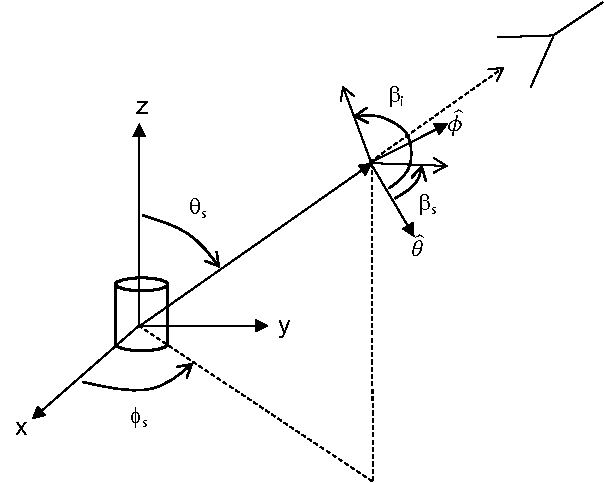
\includegraphics[width=3in]{Tmatrix/Figures/brcstmatrix} 
   \caption{Geometry the BRCS from a T-matrix.}
   \label{brcstmatrixfig}
\end{figure}



Using these in \eqref{rcs1} the backscatter radar cross section written in terms of scattered polarizations is
\begin{align}
\sigma_{\beta_s,\beta_i} &= \dfrac{(4\pi)^3}{k^2}\left\vert \sum_{lm}\sum_{l'm'} (-i)^{l+1} \left( \hat{\beta}_s\cdot \bb{C}_{lm}(\theta_s,\phi_s) \right)\left(T^{MM}_{lm,l'm'} (-i)^{l'} \bb{C}^*_{l'm'}(\theta_s,\phi_s)  - T^{MN}_{lm,l'm'} (-i)^{l'+1}  \bb{B}^*_{l'm'}(\theta_s,\phi_s)  \right)\cdot \hat{\beta}_i  \right. \nonumber \\
\ &  \left. + (-i)^{l}  \left(  \hat{\beta}_s\cdot\bb{B}_{lm}(\theta_s,\phi_s)\right)\left(T^{NM}_{lm,l'm'} (-i)^{l'} \bb{C}^*_{l'm'}(\theta_s,\phi_s)  - T^{NN}_{lm,l'm'} (-i)^{l'+1} \bb{B}^*_{l'm'}(\theta_s,\phi_s)  \right)\cdot   \hat{\beta}_i   \right\vert^2 \label{tmatrixbrcs2} 
\end{align}


The routine \texttt{brcs\_from\_Tmatrix} computes the backscatter radar cross section using \eqref{tmatrixbrcs2}. It takes as input the four block T-matrices sized $N \times N$ with harmonics up to degree $L$ all $m$ linearly indexed. The routine takes the scattered directions $(\theta_s,\phi_s)$ measured in the frame of the object, which can be any size. There are two modes: 1) if a single combination of polarization angles $\beta_i$ and $\beta_s$ is provided, then there is one output BRCS, 2) if the four $\hat{\theta}$ and $\hat{\phi}$ orthogonal BCRS vector combinations are requested, then the polarization angles are not needed. The outputs are the size of the angle arrays. The results match the analytical results for PED and dielectric spheres (see next sections).

{\scriptsize
\VerbatimInput{\code/Tmatrix/brcs_from_Tmatrix.m}
}



%
%Next we can ask what are the polarization and orientation averaged backscatter radar cross sections for co- and cross-polarizations.  These are given by 
%\ea{\left< \sigma_{co} \right> &=&  \dfrac{1}{2\pi} \int_0^{2\pi}\left(  \dfrac{1}{4\pi} \int \sigma_{\beta,\beta}(\hat{k}_i) d\Omega_i \right) d\beta \\
%\left< \sigma_{cross} \right> &=&  \dfrac{1}{2\pi} \int_0^{2\pi}\left(  \dfrac{1}{4\pi} \int \sigma_{\beta+\pi/2,\beta}(\hat{k}_i) d\Omega_i \right) d\beta }

%It appears quite complicated to continue analytically from \eqref{tmatrixbrcs1} and no simple reduction has been found yet. 





%In the backscatter direction $\theta_s = \pi-\theta_i$ and $\phi_s = \pi+\phi_i$.  Using these in \eqref{scattmatrix1} together with the parity relations for these vector spherical harmonics, \eqref{Blmparity} and \eqref{Clmparity}, we have
%\ea{\bb{E}_s(\hat{k}_s) &=& 4\pi\dfrac{e^{ikr}}{kr}  \sum_{lm}\sum_{l'm'} i^{-l-1} (-1)^{l}\bb{C}_{lm}(\theta_i,\phi_i)\left(T^{MM}_{lm,l'm'} i^{l'}  \bb{C}^*_{l'm'}(\theta_i,\phi_i)  + T^{MN}_{lm,l'm'} i^{l'+1}  \bb{B}^*_{l'm'}(\theta_i,\phi_i)  \right)\cdot  \bb{E}_i   \nonumber \\
%\ & \ &  + i^{-l}   (-1)^{l+1} \bb{B}_{lm}(\theta_i,\phi_i)\left(T^{NM}_{lm,l'm'} i^{l'}  \bb{C}^*_{l'm'}(\theta_i,\phi_i)  + T^{NN}_{lm,l'm'} i^{l'+1}  \bb{B}^*_{l'm'}(\theta_i,\phi_i)  \right)\cdot  \bb{E}_i    }
%
%The vector components in the place of the scattered direction are now identical to those in the incident direction. Let the incident and scattered polarizations be written in terms of the spherical unit vectors relative to the incident direction, with two separate angles, $\beta_i$ and $\beta_s$, 
%\ea{\hat{\beta}_i &=& \cos\beta_i \hat{\theta} + \sin\beta_i \hat{\phi} \\
%\hat{\beta}_s &=& \cos\beta_s \hat{\theta} + \sin\beta_s \hat{\phi} }
%
%The backscatter cross section given in terms of polarizations measured from the view of the incident direction is
%\ea{\sigma_{\beta_s,\beta_i} &=& \dfrac{(4\pi)^3}{k^2}\left\vert \sum_{lm}\sum_{l'm'} i^{-l-1} (-1)^{l}\hat{\beta}_s\cdot \bb{C}_{lm}(\theta_i,\phi_i)\left(T^{MM}_{lm,l'm'} i^{l'}  \bb{C}^*_{l'm'}(\theta_i,\phi_i)  + T^{MN}_{lm,l'm'} i^{l'+1}  \bb{B}^*_{l'm'}(\theta_i,\phi_i)  \right)\cdot \hat{\beta}_i  \right. \nonumber \\
%\ & \ &  \left. + i^{-l}   (-1)^{l+1} \hat{\beta}_s\cdot\bb{B}_{lm}(\theta_i,\phi_i)\left(T^{NM}_{lm,l'm'} i^{l'}  \bb{C}^*_{l'm'}(\theta_i,\phi_i)  + T^{NN}_{lm,l'm'} i^{l'+1}  \bb{B}^*_{l'm'}(\theta_i,\phi_i)  \right)\cdot   \hat{\beta}_i   \right\vert^2 }






\clearpage
\newpage
\subsection{Backscatter Radar Cross Section of a Sphere}

%\noindent where $\bb{E}_s$ is the far-field scattered field, $\bb{E}_i $ are plane waves incident on the target, and $\hat{p}$ and $\hat{q}$ are polarization unit vectors. 

For a sphere, the radar backscatter is independent of the incident direction, and \eqref{scattmatrix1} can be simplified analytically.  Let the incident direction be in the $+\hat{z}$ direction, $(\theta_i,\phi_i) = (0,0)$, and the scattered direction be $-\hat{z}$ with $(\theta_i,\phi_i) = (\pi,0)$.  Let the incident and scattered electric field have both $\hat{x}$ and $\hat{y}$ components   
\eq{\bb{E}_i = E_x \hat{x} + E_y \hat{y}}

%\ea{\bb{E}_s(\br) &=& 4\pi\dfrac{e^{ikr}}{kr}  \sum_{lm}\sum_{l'm'} \nonumber \\
%\ & \ & i^{-l-1} \bb{C}_{lm}(\pi,0)\left(T^{MM}_{lm,l'm'} i^{l'}  \bb{C}^*_{l'm'}(0,0)  + T^{MN}_{lm,l'm'} i^{l'+1}  \bb{B}^*_{l'm'}(0,0)  \right)\cdot  \bb{E}_i   + \nonumber \\
%\ & \ &  i^{-l}   \bb{B}_{lm}(\pi,0)\left(T^{NM}_{lm,l'm'} i^{l'}  \bb{C}^*_{l'm'}(0,0)  + T^{NN}_{lm,l'm'} i^{l'+1}  \bb{B}^*_{l'm'}(0,0)  \right)\cdot  \bb{E}_i  \nonumber \\ }


For a PEC or dielectric sphere, the T-matrix is diagonal with zero cross terms so that \eqref{scattmatrix} reduces to one sum as 
\ea{\bb{E}_s(\pi,0) &=& -4\pi i\dfrac{e^{ikr}}{kr}   \sum_{lm}\bb{C}_{lm}(\pi,0)T^{MM}_{lm} \bb{C}^*_{lm}(0,0) \cdot  \bb{E}_i   -  \bb{B}_{lm}(\pi,0)T^{NN}_{lm}  \bb{B}^*_{lm}(0,0) \cdot  \bb{E}_i  }

%\ea{\bb{E}_s(\br) &=& 4\pi\dfrac{e^{ikr}}{kr}  \sum_{lm}\nonumber \\
%\ & \ & i^{-l-1} \bb{C}_{lm}(\pi,0)\left(T^{MM}_{lm} i^{l}  \bb{C}^*_{lm}(0,0) \right)\cdot  \bb{E}_i   + \nonumber \\
%\ & \ &  i^{-l}   \bb{B}_{lm}(\pi,0)\left( T^{NN}_{lm} i^{l+1}  \bb{B}^*_{lm}(0,0)  \right)\cdot  \bb{E}_i  \nonumber \\ }
Using \eqref{clmzplus}, \eqref{blmzplus}, \eqref{clmzminus}, \eqref{blmzminus}, this reduces to
\ea{\bb{E}_s(\pi,0) &=& \dfrac{-i}{2} \dfrac{e^{ikr}}{kr}  \sum_{l} (-1)^l (2l+1) \left[ \hat{x} (T^{MM}_{l} - T^{NN}_{l}) E_x - \hat{y} (T^{MM}_{l} - T^{NN}_{l}) E_y\right]\label{esbacksphere} }

This shows that the scattered field in the backscatter direction of a sphere is polarization independent with no cross-pol. Substituting \eqref{esbacksphere} into \eqref{rcs1} and choosing either polarization, the polarization amplitude will cancel. The backscatter radar cross section of a sphere where only the diagonal elements of the T-matrix are non-zero
\eq{\sigma = \dfrac{\pi}{k^2} \left\vert \sum_{l=1}^{\infty} (-1)^l (2l+1) \left(T^{MM}_{l} - T^{NN}_{l}\right) \right\vert^2 \label{rcssphere}}

\subsection{Backscatter RCS of a PEC Sphere}

Substituting the T-matrix for a PEC sphere into \eqref{rcssphere}, the backscatter RCS of a PEC sphere is
\eq{\sigma_{PEC} = \dfrac{\pi}{k^2} \left\vert \sum_{l=1}^{\infty} (-1)^l (2l+1) \left(\dfrac{j_l(ka)}{h_l^{(1)}(ka)}  - \dfrac{[k a j_l(ka)]'}{[k a h_l^{(1)}(ka)]'}\right) \right\vert^2 \label{sigmapec}}


%
%Using the Wronskian
%\eq{j_l(x) {h'}_l^{(1)}(x) - h_l^{(1)}(x) j_l'(x) = \dfrac{i}{x^2} }
%
%\eq{\sigma_{PEC} = \dfrac{\pi}{k^2} \left\vert \sum_{l=1}^{\infty} \dfrac{(-1)^l (2l+1) }{ ka h_l^{(1)}(ka) [k a h_l^{(1)}(ka)]'} \right\vert^2 }
%
%Next, we write this in terms of logarithmic derivative of the Bessel functions.  Let $\chi$ be the Riccati-Bessel function or Riccati-Hankel function.  The logarithmic derivative is 
%
%\eq{\phi_n(x) = x j_n(x)}
%\eq{\zeta_n(x) = xh_n^{(1)}(x)}
%
%\eq{A_n = \dfrac{1}{x j_n(x)}\dd{x j_n(x)}{x}  }
%\eq{B_n = \dfrac{1}{xh_n^{(1)}(x)}\dd{xh_n^{(1)}(x)}{x}}
%
%\eq{\chi_l(x) = xz_l(x)}
%\eq{C_l = \dfrac{1}{\chi_l}\dd{\chi_l}{x} }
%
%These have the single term recurrence 
%
%\eq{\rho_l = \dfrac{\chi_l}{\chi_{l+1}}}
%\eq{\dfrac{1}{\rho_l} = \dfrac{2l+1}{x} - \rho_{l-1}}
%\eq{C_l = -\dfrac{l}{x} + \dfrac{1}{\dfrac{l}{x} - C_{l-1}}}
%
%Using the fact that
%\ea{j_0(x) &=& \dfrac{\sin x}{x} \\
%j_1(x) &=& -\dfrac{\cos x}{x} + \dfrac{\sin x}{x^2} \\
%h_0^{(1)}(x) &=& \dfrac{e^{i x}}{ix} \\
%h_1^{(1)}(x) &=& -\left(1 + \dfrac{i}{x}\right) \dfrac{e^{i x}}{x} }
%
%\eq{\psi_0 = \dfrac{e^{ix}}{i}}
%\eq{\rho_0 = \dfrac{x}{1 - ix}}
%\eq{C_0 = 1 + i - \dfrac{1}{x}}
%
%
%
%
%\eq{\sigma_{PEC} = \dfrac{\pi}{k^2} \left\vert \sum_{l=1}^{\infty} \dfrac{(-1)^l (2l+1) }{\chi_l^2 C_l  } \right\vert^2 }


%
%
%\eq{z'_l(x) = z_{l-1}(x) - \dfrac{l}{x}z_{l}(x) }
%this becomes
%\eq{\sigma_{PEC} = \dfrac{\pi}{k^2} \left\vert \sum_{l=1}^{\infty} \dfrac{(-1)^l (2l+1) }{ x h_l^{(1)}(x)\left((1-l)h_l^{(1)}(x) + x h_{l-1}^{(1)}(x)\right) } \right\vert^2 }
%
%$x = ka$.  The Hankel function can be computed recursively as 
%\eq{z_l(x) = \dfrac{2(l-1)}{x} z_{l-1}(x) - z_{l-2}(x)}
%
%with initial conditions
%\ea{h_0^{(1)}(x) &=& \dfrac{e^{i x}}{ix} \\
%h_1^{(1)}(x) &=& -\left(1 + \dfrac{i}{x}\right) \dfrac{e^{i x}}{x} }


\begin{figure}[H] 
   \centering
   \includegraphics[width=3.5in]{Tmatrix/Figures/brcspecsphere} 
   \caption{RCS of PEC sphere, normalized by cross-section area.  The maximum occurs at $ka \approx 1.03$, with a value of about 3.65 (linear).}
\end{figure}


The routine \texttt{brcs\_pec\_sphere} is a workable routine to compute \eqref{sigmapec}. The sum is truncated when incremental change is less than machine precision. The standard and better way to compute this is to use logarithmic derivatives of the Bessel functions, but that is a separate topic.

{\footnotesize
\VerbatimInput{\code/Tmatrix/brcs_pec_sphere.m}
}

\subsection{Backscatter RCS of a Dielectric Sphere}

Using the T-matirx for the dielectric sphere in \eqref{rcssphere}, the backscatter RCS of a non-magnetic dielectric sphere is 
\eq{\sigma = \dfrac{\pi}{k^2} \left\vert \sum_{l=1}^{\infty} (-1)^l (2l+1) \left(\dfrac{j_2 j_1'  -  j_1j_2'}{ h_1 j_2' -  j_2 h_1'} - \dfrac{ x_2^2 j_2 j_1' -  x_1^2 j_1 j_2' }{ x_1^2 h_1 j_2' - x_2^2  j_2 h_1' } \right) \right\vert^2 \label{sigmaer}}

which uses the shorthand: 
\ea{x_1 &=& k_1 a \\
x_2 &=& k_2 a \\
j_1 &=& j_l(k_1a) \\
j_1' &=& [k_1 a j_l(k_1a)]' \\
j_2 &=& j_l(k_2a) \\
j_2' &=& [k_2 a j_l(k_2a)]' \\
h_1 &=& h_l^{(1)}(k_1a) \\
h_1' &=& [k_1 a h_l^{(1)}(k_1a)]' 
}

\noindent where $k_1$ is the wavenumber outside the sphere, and $k_2$ is wavenumber inside the sphere.  Making use of the Wronskian $j_l(x) {h'}_l^{(1)}(x) - h_l^{(1)}(x) j_l'(x) = i/x^2$, it can be shown that $h_1' j_1 - h_1 j_1'  = i/x_1$.  Then the backscatter can also be written 
\eq{\sigma = \dfrac{\pi}{k^2} \left\vert \sum_{l=1}^{\infty} (-1)^l (2l+1) \left(\dfrac{j_2 j_2' ( x_2^2 - x_1^2) }{x_1 \left(h_1 j_2' - j_2 h_1' \right)\left(x_1^2 h_1 j_2' - x_2^2  j_2 h_1' \right)}\right) \right\vert^2 }

\clearpage
\begin{figure}[h] 
   \centering
   \subfigure{\includegraphics[width=3.2in]{Tmatrix/Figures/brcsdielectricsphere}  \label{brcsdiesph} } 
   \subfigure{\includegraphics[width=3.1in]{Tmatrix/Figures/brcsdielectricspheregrid}   \label{brcsdiesphall}}
   \caption{Backscatter RCS of dielectric sphere, normalized by cross-section area, in free-space. Left: $\epsilon_r = 2.5$. Right: $\epsilon_r =$1 to 5, and $a/\lambda_o$ = 0 to 2.}
 \end{figure}
 
 
%\begin{figure}[h] 
%   \centering
%   \includegraphics[width=3.5in]{Tmatrix/Figures/brcsdielectricsphere} 
%   \caption{Backscatter RCS of dielectric sphere, normalized by cross-section area, in free-space.  $\epsilon_r = 2.5$.}
%   \label{brcsdiesph}
%\end{figure}
%
%\begin{figure}[h] 
%   \centering
%   \includegraphics[width=3.5in]{Tmatrix/Figures/brcsdielectricspheregrid} 
%   \caption{Backscatter RCS of lossless dielectric sphere, normalized by cross-section area, in free-space.}
%      \label{brcsdiesphall}
%\end{figure}

The routine \texttt{brcs\_dielectric\_sphere} is a workable routine for the computation of \eqref{sigmaer}.  Assuming a background of vacuum, Figure \ref{brcsdiesph} shows the backscatter RCS for a sphere with $\epsilon_r = 2.5$ as a function of sphere radius. Figure \ref{brcsdiesphall} shows the same as a function of $k_o a$ and $\epsilon_r$. 

{\footnotesize
\VerbatimInput{\code/Tmatrix/brcs_dielectric_sphere.m}
}

\clearpage
\section{Scattering Cross Section from T-matrix}

The scattering cross section is equal to the scattered power integrated over the sphere for a unit amplitude incident electric field and specific incident direction. From \cite{tsang1985theory}, the scattering cross section is written in terms of the S-matrix as 
\eq{\sigma_{s\beta}(\hat{k}_i) = \int_S \left( \vert S_{p \beta}(\hat{k}_s,\hat{k}_i) \vert^2 + \vert S_{q \beta}(\hat{k}_s,\hat{k}_i) \vert^2 \right) d\Omega_s  }

\noindent where $\beta$ is the incident polarization and $p$ and $q$ are any two orthogonal scattered polarizations. Taking the magnitude squared of \eqref{scattmatrix1} without the terms $E_o e^{ikr}/r $, integrating this over the scattered field directions, and applying orthonormality of the vector spherical harmonics, one gets, similar to \cite{tsang1985theory},

\ea{\sigma_{s\beta}(\hat{k}_i) &=& \dfrac{16\pi^2}{k^2} \sum_{lm} \left\{ \left\vert \sum_{l'm'} \left(T^{MM}_{lm,l'm'} i^{l'}  \bb{C}^*_{l'm'}(\theta_i,\phi_i)  + T^{MN}_{lm,l'm'} i^{l'+1}  \bb{B}^*_{l'm'}(\theta_i,\phi_i)  \right)\cdot  \hat{\beta} \right\vert^2 \right. \nonumber \\
\ & \ &  +\left. \left\vert \sum_{l'm'} \left(T^{NM}_{lm,l'm'} i^{l'}  \bb{C}^*_{l'm'}(\theta_i,\phi_i)  + T^{NN}_{lm,l'm'} i^{l'+1}  \bb{B}^*_{l'm'}(\theta_i,\phi_i)  \right)\cdot  \hat{\beta} \right\vert^2 \right\}  \label{tmatrixscatcrosssection} }

The routine \texttt{compute\char`_scs\char`_from\char`_tmatrix} computes the scattering cross section of an object from its T-matrix. It takes as input the four $N \times N$ bock T-matrices where $N = L^2 + 2L$, for harmonics up to maximum degree $L$ all $m$.  The incident angles can be any size. The incident polarization is defined relative to the spherical unit vectors $\hat{\beta} = \cos \beta \hat{\theta} + \sin\beta \hat{\phi}$.  Recall $\hat{v} =\hat{\theta}$ and $\hat{h} =\hat{\phi}$. Values $\beta = [0,\pi/2]$ correspond to $v, h$ respectively. The array of $\beta$ can be any size. The scattering cross section is returned on an array with dimensions that are the concatenation of the sizes of the incident direction array and polarization angle array.  


{\footnotesize
\VerbatimInput{\code/Tmatrix/compute_scs_from_tmatrix.m}
}

% From \cite{tsang2000scattering}, if the scattered electric field is written in terms of the far field pattern as 
%\eq{\bb{E}_s = \left( \hat{v}_s E_{vs
%} + \hat{h}_s E_{hs} \right) \dfrac{e^{ikr}}{r}}
%with 
%\eq{\twobyone{E_{vs}}{E_{hs}} = \twobytwo{S_{vv}}{S_{vh}}{S_{hv}}{S_{hh}} \twobyone{E_{vi}}{E_{hi}}}
%
%then the scattering cross section for polarization $p = v,h$ and fixed incident direction is 
%\eq{\sigma_{sp}(\hat{k}_i) = \int_S \left( \vert S_{vp}(\hat{k}_s,\hat{k}_i) \vert^2 + \vert S_{hp}(\hat{k}_s,\hat{k}_i) \vert^2 \right) d\Omega_s  }

%
%\eq{\bb{E}_s = \hat{e}_s E_o f(\hat{k}_s,\hat{k}_i) \dfrac{e^{ikr}}{r}}
%
%then the scattering cross section is 
%\eq{\sigma_s = \int \left\vert f(\hat{k}_s,\hat{k}_i) \right\vert^2 d\Omega_s} 
%


\subsection{Scattering Cross Section of a Sphere}

For the scattering cross section of a sphere, from symmetry, we only need to consider one incident polarization and an arbitrary incident direction. Assume that the incident plane wave propagates in the $z$ direction:
\eq{\bb{E}_i = E_o \hat{x}  \label{Eincxz}}

The T-matrix of the sphere is diagonal with zero cross terms, which means \eqref{tmatrixscatcrosssection} simplifies to
\ea{\sigma_{s} &=& \dfrac{16\pi^2}{k^2} \sum_{lm} \left\{ \left\vert  T^{MM}_{lmlm}   \bb{C}^*_{lm}(0,0) \cdot  \hat{x} \right\vert^2 + \left\vert T^{NN}_{lmlm}  \bb{B}^*_{lm}(0,0)  \cdot  \hat{x} \right\vert^2 \right\}  }

From \eqref{clmzplus}, \eqref{blmzplus}, and \eqref{Eincxz}, the vector spherical harmonics for $z$ propagation wave have only $m=\pm1$ harmonics and the dot product with $\hat{x}$ is
\eq{\bb{C}^*_{l,\pm 1}(0,0) \cdot  \hat{x}=  \dfrac{i}{2} \sqrt{\dfrac{2l+1}{4\pi}} }
\eq{\bb{B}^*_{l,\pm 1}(0,0) \cdot  \hat{x} = \pm  \dfrac{1}{2} \sqrt{\dfrac{2l+1}{4\pi}} }

Substituting these we get 
%\ea{\sigma_{sx}(\hat{k}_i) &=& \dfrac{16\pi^2}{k^2} \sum_{lm} \left\{ \left\vert  T^{MM}_{lmlm}   \bb{C}^*_{lm}(0,0) \cdot  \hat{x} \right\vert^2 + \left\vert T^{NN}_{lmlm}  \bb{B}^*_{lm}(0,0)  \cdot  \hat{x} \right\vert^2 \right\}  }

% scattered field is 
%\ea{\bb{E}_s(\hat{k}_s) &=& 4\pi\dfrac{e^{ikr}}{kr} i  \sum_{lm}-\bb{C}_{lm}(\theta_s,\phi_s)T^{MM}_{lm} \bb{C}^*_{lm}(0,0) \cdot  \bb{E}_i   +  \bb{B}_{lm}(\theta_s,\phi_s)T^{NN}_{lm}  \bb{B}^*_{lm}(0,0) \cdot  \bb{E}_i  \nonumber \\ }
%
%Using \eqref{clmzplus}, \eqref{blmzplus}, and \eqref{Eincxz}
%
%\eq{\bb{C}^*_{l,\pm 1}(0,0) \cdot  \bb{E}_i = E_o \dfrac{i}{2} \sqrt{\dfrac{2(l+1)}{4\pi}} }
%\eq{\bb{B}^*_{l,\pm 1}(0,0) \cdot  \bb{E}_i = \pm E_o \dfrac{1}{2} \sqrt{\dfrac{2(l+1)}{4\pi}} }
%
%\ea{\bb{E}_s(\hat{k}_s) &=& E_o 4\pi\dfrac{e^{ikr}}{2kr} \sum_{l,m=\pm1} \sqrt{\dfrac{2(l+1)}{4\pi}} \left( \bb{C}_{lm}(\theta_s,\phi_s)T^{MM}_{lm}    \pm i \bb{B}_{lm}(\theta_s,\phi_s)T^{NN}_{lm}  \right) \nonumber \\ }
%%\ea{\bb{E}_s(\br) &=& E_o 4\pi\dfrac{e^{ikr}}{2kr} \sum_{l} \sqrt{\dfrac{2(l+1)}{4\pi}} \left( (\bb{C}_{l,1}(\theta,\phi) + \bb{C}_{l,-1}(\theta,\phi)) T^{MM}_{l}    + i \left( \bb{B}_{l,1}(\theta,\phi) + \bb{B}_{l,-1}(\theta,\phi)\right) T^{NN}_{l}  \right) \nonumber \\ }
%
%Dropping $E_o$ and $e^{ikr}/r$, integrating the magnitude squared of the scattered field over the sphere, 
%
%\ea{\sigma_{sca} &=& \left(\dfrac{4\pi}{2k}\right)^2  \int \left\vert \sum_{l} \sqrt{\dfrac{2(l+1)}{4\pi}} \left( (\bb{C}_{l,1}(\theta_s,\phi_s) + \bb{C}_{l,-1}(\theta_s,\phi_s)) T^{MM}_{l}   \right.\right. \nonumber \\
%\ & \ & \left.\left. + i \left( \bb{B}_{l,1}(\theta_s,\phi_s) + \bb{B}_{l,-1}(\theta_s,\phi_s)\right) T^{NN}_{l}  \right) \right\vert^2 d\Omega_s }
%
%Expanding the magnitude squared as two conjugate independent sums, then after applying orthogonality of the vector spherical harmonics each term becomes independent.  

\eq{\sigma_{s} = \dfrac{2\pi}{k^2}  \sum_{l=1}^{\infty}(2l+1) \left(\left\vert T^{MM}_{l} \right\vert^2 + \left\vert T^{NN}_{l} \right\vert^2  \right) \label{spheresca}  }

A factor of two comes from summing the $m=\pm1$ terms. 

\subsection{Scattering Cross Section of a PEC Sphere}

The scattering cross section of a PEC sphere is given by substituting the T-matrix for a PEC sphere into \eqref{spheresca}
\eq{\sigma_{s,PEC} = \dfrac{2\pi}{k^2}  \sum_{l=1}^{\infty}(2l+1) \left(\left\vert \dfrac{j_l(ka)}{h_l^{(1)}(ka)}  \right\vert^2 + \left\vert \dfrac{[k a j_l(ka)]'}{[k a h_l^{(1)}(ka)]'} \right\vert^2  \right) \label{scspecsphere}}

\noindent where the sphere has radius $a$ in a background with wavenumber $k$.

\begin{figure}[H] 
   \centering
   \includegraphics[width=4in]{Tmatrix/Figures/scspecsphere} 
   \caption{Scattering cross section of a PEC sphere, normalized by cross-section area, in free-space.}
   \label{scspecsph}
\end{figure}




The routine \texttt{scs\char`_pec\char`_sphere} is a workable routine to compute \eqref{scspecsphere}. The sum is truncated when incremental change is less than machine precision. 

{\footnotesize
\VerbatimInput{\code/Tmatrix/scs_pec_sphere.m}
}
\clearpage
\subsection{Scattering Cross Section of a Dielectric Sphere}

The scattering cross section of a dielectric sphere is given by substituting the T-matrix for a dielectric sphere into \eqref{spheresca}. This gives identical results to \cite{tsang2000scattering} Figure 1.6.3 and also matches outputs from Ulaby and Long 2014 Code Module 8.12.


\begin{figure}[H] 
   \centering
   \includegraphics[width=3.5in]{Tmatrix/Figures/scsdielectricspheregrid} 
   \caption{Scattering cross section of lossless dielectric sphere, normalized by cross-section area, in free-space.}
      \label{scsdiesphall}
\end{figure}


The routine \texttt{scs\char`_dielectric\char`_sphere} computes the scattering cross section of a dielectric sphere given the inner and outer wavenumbers $k_1$, $k_2$, and sphere radius $a$.  

{\scriptsize
\VerbatimInput{\code/Tmatrix/scs_dielectric_sphere.m}
}

%
%\subsection{Rayleigh Limit}
%
%Classical Rayleigh scattering comes by taking the small argument limit of \eqref{spheresca}.  Keeping only the $l=1$ term, assuming nonmagnetic.  Using the facts that 
%
%\ea{j_n(x) & \approx & \dfrac{x^n}{1 \cdot 3 \cdot 5 \cdots(2n+1)} \\
%h_n^{(1)}(x) & \approx &  \dfrac{x^n}{1 \cdot 3 \cdot 5 \cdots(2n+1)} -i \dfrac{1 \cdot 3 \cdot 5 \cdots(2n-1)}{x^{n+1}} }
%
%Then it can be shown that 
%\ea{ \lim_{x \rightarrow 0} j_1(x) & \approx & \dfrac{x}{3}\\
% \lim_{x \rightarrow 0} (x j_1(x))' & \approx &  \dfrac{2x}{3} \\
% \lim_{x \rightarrow 0} h_1^{(1)}(x) &  \approx & \dfrac{x}{3} -i x^{-2}  \\
% \lim_{x \rightarrow 0} (x h_1^{(1)}(x) )' & \approx &  i x^{-2} + \dfrac{2x}{3} }
%
%Using 
%\ea{x_1 &=& k_1 a \\
%x_2 &=& k_2 a}
%
%and substituting the limits
%\ea{T_{lmlm}^{MM} &=& \dfrac{ \dfrac{x_2}{3} \dfrac{2x_1}{3} -   \dfrac{x_1}{3}\dfrac{2x_2}{3}}{  \left(\dfrac{x_1}{3} -i x_1^{-2}\right) \dfrac{2x_2}{3} -   \dfrac{x_2}{3} \left( i x_1^{-2} + \dfrac{2x_1}{3} \right) } \\
%T_{lmlm}^{NN} &=& \dfrac{x_2^2 \dfrac{x_2}{3} \dfrac{2x_1}{3} -   x_1^2\dfrac{x_1}{3} \dfrac{2x_2}{3} }{  x_1^2 \left(\dfrac{x_1}{3} -i x_1^{-2} \right) \dfrac{2x_2}{3} -  x_2^2  \dfrac{x_2}{3}\left( i x_1^{-2} + \dfrac{2x_1}{3} \right) } } 
%
%
%\ea{T_{lmlm}^{MM} &=& \dfrac{  j_l(x_2) [x_1 j_l(x_1)]' -   j_l(x_1)[x_2 j_l(x_2)]'}{  h_l^{(1)}(x_1) [x_2 j_l(x_2)]' -   j_l(x_2) [x_1 h_l^{(1)}(x_1)]'}  \\
%T_{lmlm}^{NN} &=& \dfrac{x_2^2 j_l(x_2) [x_1 j_l(x_1)]' -   x_1^2j_l(x_1) [x_2 j_l(x_2)]' }{  x_1^2 h_l^{(1)}(x_1) [x_2j_l(x_2)]' -  x_2^2  j_l(x_2)[x_1 h_l^{(1)}(x_1)]'} } 
%
%
%\subsection{Scattering Efficiency of a Dielectric Sphere}
%
%In general, the scattering efficiency is defined as the scattering cross section divided by the geometric cross section. For a sphere of radius $a$ this is
%
%\eq{Q_{sca} = \dfrac{\sigma_{sca}}{\pi a^2} }
%
%This is a measure of the amount of power scattered compared to the power intercepted. For a sphere in the Mei regime, this value is around 2 and can be as high as 4.  This is means that the scattering cross section for large spheres near resonances is greater than the geometric cross section.  
%
%This is given by the simple routine \texttt{scatEfficiencyDieletricSphere}.
%
%{\footnotesize
%\VerbatimInput{\code/Tmatrix/scatEfficiencyDieletricSphere.m}
%}

\clearpage

\subsection{Polarization and Orientation Averaged Scattering Cross Section using T-matrix}

We can compute the polarization and orientation averaged scattering cross section directly from the elements of the T-matrix using \eqref{polorientavescs} and \eqref{tmatrixscatcrosssection}:
\ea{\left< \sigma \right> &=&  \dfrac{1}{2\pi} \int_0^{2\pi}\left(  \dfrac{1}{4\pi} \int \sigma_{s\beta}(\hat{k}_i) d\Omega_i \right) d\beta }

Let the incident polarization vector be $\hat{\beta} = \cos \beta \hat{\theta} + \sin\beta \hat{\phi}$, then, for example, the first magnitude squared term in \eqref{tmatrixscatcrosssection} looks like
\ea{I_{lm}(\theta_i,\phi_i,\beta) &=& \left\vert \sum_{l'm'}  T^{MM}_{lm,l'm'} i^{l'}  \left(C^*_{\theta,l'm'}(\theta_i,\phi_i) \cos\beta + C^*_{\phi,l'm'}(\theta_i,\phi_i) \sin\beta \right) \right. \nonumber \\
\ & \  & +\left. T^{MN}_{lm,l'm'} i^{l'+1} \left(B^*_{\theta,l'm'}(\theta_i,\phi_i) \cos\beta + B^*_{\phi,l'm'}(\theta_i,\phi_i) \sin\beta \right)  \right\vert^2 }

After expanding the magnitude squared with a second sum, it is clear that cross terms having $\cos\beta\sin\beta$ will not survive the $\beta$ integral and can be ignored. From orthogonality of the vector spherical harmonics the cross terms of the vector spherical harmonics will not survive the integration over incident directions. The only terms that matter are of the form $C^*_{\theta,l'm'}(\theta_i,\phi_i)C_{\theta,l''m''}(\theta_i,\phi_i) \cos^2\beta + C^*_{\phi,l'm'}(\theta_i,\phi_i)C_{\phi,l''m''}(\theta_i,\phi_i) \sin^2\beta $. The trick is to first compute the $\beta$ integral, so that $\cos^2\beta$ and $\sin^2\beta$ become $\pi$ which is factored out, after which $1/2$ remains from the $\beta$ integral normalization. The dot products of the vector spherical harmonics then integrate to 1 and collapse one sum. Only the $1/4\pi$ remains from the normalization of the integral over incident directions. The end result is a double sum over the magnitude squared of all elements of the T-matrix:
\eq{\left< \sigma \right> =   \dfrac{2\pi}{k^2} \sum_{lm}\sum_{l'm'} \left\vert T^{MM}_{lm,l'm'} \right\vert^2 + \left\vert T^{MN}_{lm,l'm'} \right\vert^2  + \left\vert T^{NM}_{lm,l'm'} \right\vert^2  + \left\vert T^{NN}_{lm,l'm'} \right\vert^2  \label{tmatrixpolorientave}}

Equation \eqref{tmatrixpolorientave} is basically the square of the Frobenius norm of the entire T-matrix, scaled by a constant that depends on wavelength. This expression is amazingly elegant and comes from the fact that each T-matrix element contains scattering information for all spherical directions and polarizations at once. This can be checked against the scattering cross section of the sphere, which is independent of incident polarization and direction, and therefore $\left< \sigma \right> = \sigma_s$: the T-matrix elements of the sphere are diagonal (eliminates one sum) with no cross terms and depends only on $l$, so that each sum over $m$ contributes $2l+1$ terms, which gives \eqref{spheresca}.  

The routine \texttt{compute\char`_avescs\char`_from\char`_tmatrix}  computes the polarization and orientation average scattering cross section from a T-matrix. It takes as input the four $N \times N$ block T-matrices where $N = L^2 + 2L$, for harmonics up to maximum degree $L$ all $\pm m$ and returns \eqref{tmatrixpolorientave}. This is easy enough to compute.


{\footnotesize
\VerbatimInput{\code/Tmatrix/compute_avescs_from_tmatrix.m}
}


